%% ------------------------------------------------------------------------- %%
\chapter{Experimental Analysis}
\label{cap:experimental-analysis}

Each dataset pipeline result has all evaluated metrics (AUC, Brier and Logloss), the dataset statistics (described in \ref{dataset-aggregated-statistics}) and the generated hyperparameter space according to Section \ref{sec:hyperparam-space} of Chapter \ref{cap:study-methodology}.

The focus of this Chapter is to give an overview of the main experimental analysis, how the datasets were clustered and a basic explanation of the statistical theory necessary for the analysis and statistical framework used.


%% ------------------------------------------------------------------------- %%
\section{Single Dataset Experiment}
\label{sec:single-dataset}

Each dataset result in the study has the following files:

\begin{enumerate}
    \item \textbf{\code{shape}}: The number of data points $D_i$ and the number of features of both train and test set;
    \item \textbf{\code{analyzer\_info}}: A dictionary with information calculated by the \code{analyzer}. It contains the feature set, what is the target column, an indicator if the dataset contains any categorical variable, and all the categorical features if it has any;
    \item \textbf{\code{openml\_object}}: The original \textit{OpenML} object of the dataset, with its name, description (if it has one), basic attribute information, etc;
    \item \textbf{\code{hp\_tree}}: The generated hyperparameter tree for the dataset, i.e. all nodes of $Hspace_i$;
    \item \textbf{\code{final\_result}}: All the metric results for all combinations of hyperparameters in the hyperparameter tree; Contains the values used for the main analysis.
\end{enumerate}

Each entry of \code{final\_result} contains the evaluators result for both train and test set for all hyperparameters combinations. An example of a single entry in the \code{final\_result} for a specific dataset (\textit{BNG(kr-vs-kp)}, a chess move classification problem) is shown in \ref{lst:krkp-result}.

\begin{lstlisting}[caption={BNG(kr-vs-kp) experiment result for hyperparam combination (0.3, 1700, 10)}, label={lst:krkp-result}]
{'learning_rate': 0.30000000000000004,
'num_estimators': 1700,
'max_depth': 10,
'num_leaves': 1023,
'seed': 42,
'nthread': 32,
'verbose': -1,
'train_result': {'auc_evaluator__target': 0.9963452091395292,
    'logloss_evaluator__target': 0.07025840176806959,
    'brier_score_evaluator__target': 0.020611611004153745},
'test_result': {'auc_evaluator__target': 0.9857593012343584,
    'logloss_evaluator__target': 0.208979460099794,
    'brier_score_evaluator__target': 0.03484311126894392},
}  \end{lstlisting}


Since each dataset has multiple results assigned to it, one can do an \textbf{individual analysis} looking into a single dataset behavior. In this section, a summarized analysis of the \textbf{BNG(kr-vs-kp)} dataset is given as an example. The \textit{BNG(kr-vs-kp)} or "King+Rook versus King+Pawn" is one of the datasets available in the OpenML platform, where the objective is to classify if the white player can win or not (given the board positions determined by the feature values), and it is described in more details in \cite{shapiro1987structured}. The "BNG" means this is an artificially augmented/generated dataset.

\subsection{Individual Hyperparameter Impact}
\label{subsec:indv-impact}

The first node of the hyperparameter tree only defines single hyperparameters values. By keeping the default LightGBM values for the remaining hyperparameters one can observe the impact of changing a single hyperparameter on each metric of interest. The plot of these values is the classical learning curve used in model tuning to assess the hyperparameter effect on model performance. In the Figure \ref{fig:res-ind2} impact of max depth is illustrated and in \ref{fig:res-ind1} the number of estimators, for the \textit{BNG(kr-vs-kp)} dataset.

\begin{figure}[!h]
    \centering
    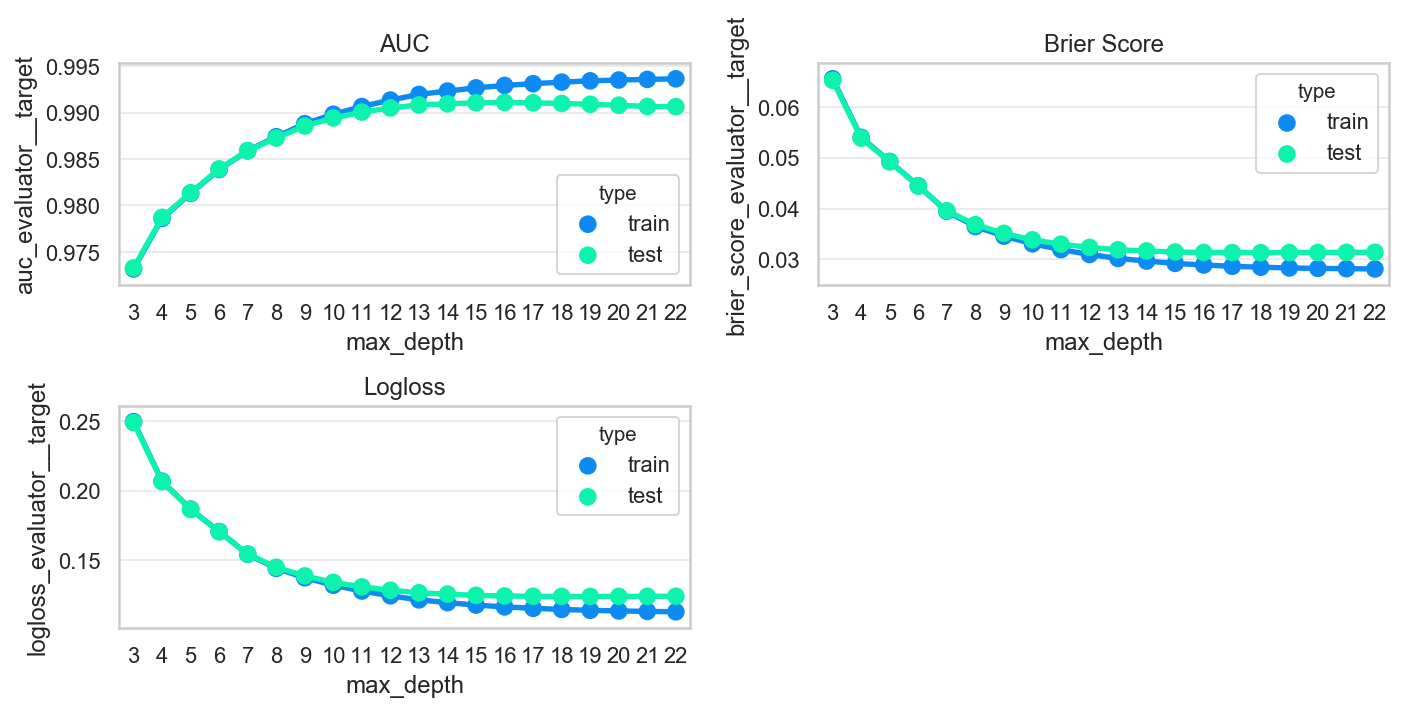
\includegraphics[width=1\textwidth]{res-ind2.png} 
    \caption{Individual impact of \textbf{\code{max\_depth}} on the \textit{BNG(kr-vs-kp)} dataset: one can observe that when $max\_depth > 14$ the model starts to overfit.}
    \label{fig:res-ind2}
\end{figure}

\begin{figure}[!h]
    \centering
    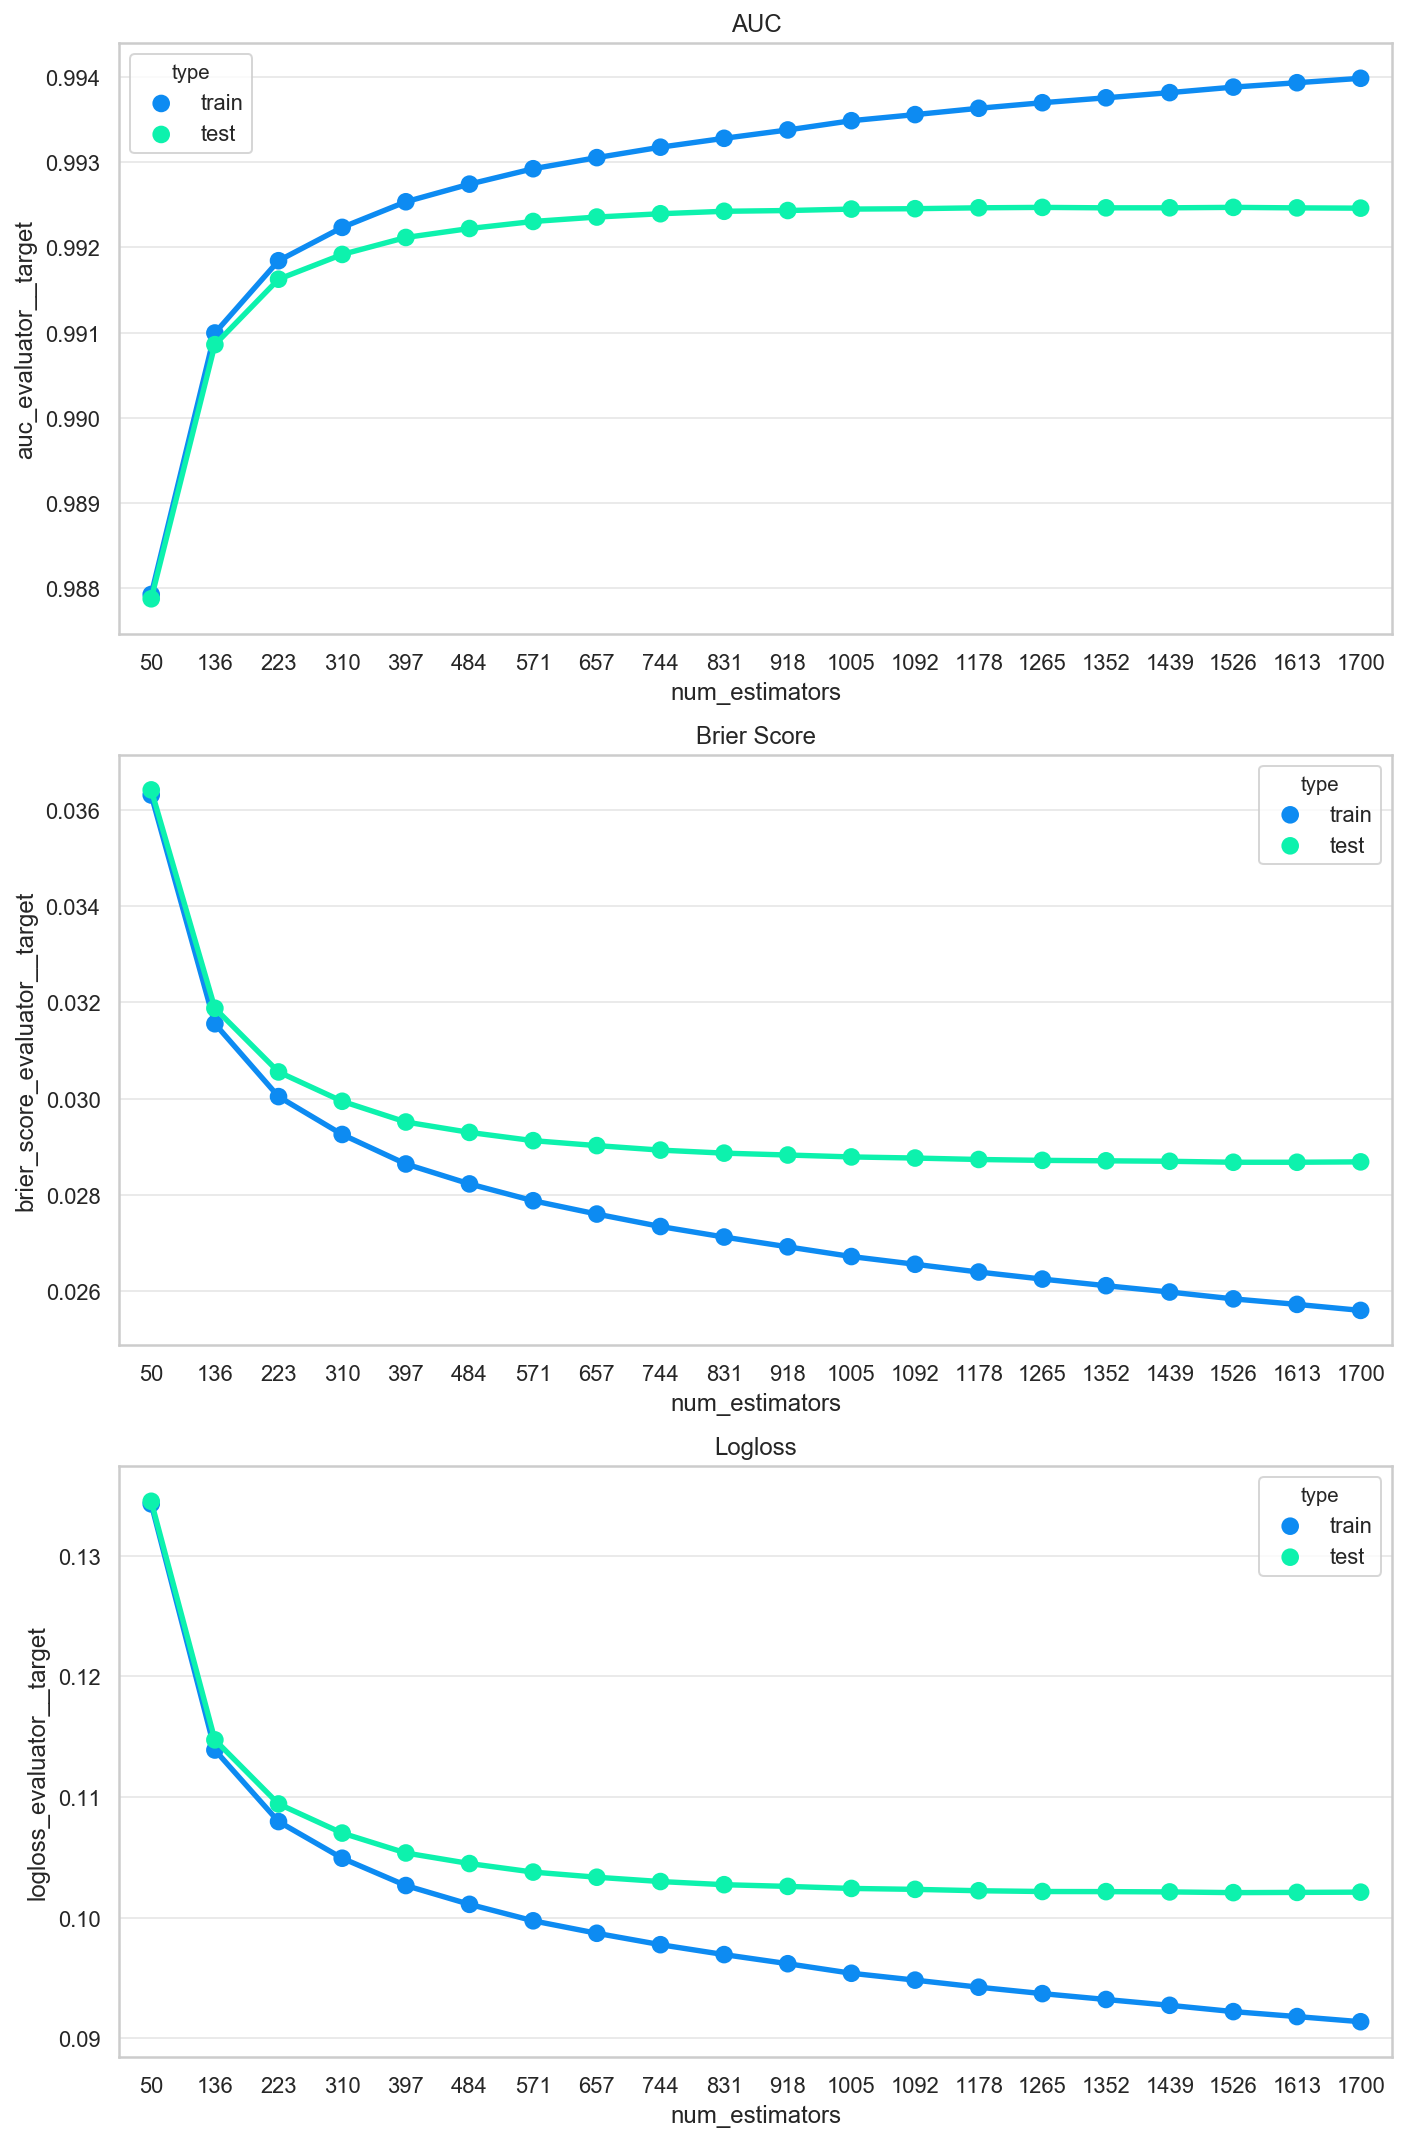
\includegraphics[width=1\textwidth, height=1.2\textwidth]{res-ind1.png} 
    \caption{Individual impact of \textbf{\code{num\_estimators}} on the \textit{BNG(kr-vs-kp)} dataset}
    \label{fig:res-ind1}
\end{figure}

\subsection{Hyperparameter Pairs Impact}
\label{subsec:double-impact}

The second node of the hyperparameter tree defines all pairs of possible combinations of hyperparameters. In this study, these combinations are $MD_i \times LR_i$, $MD_i \times NE_i$ and $LR_i \times NE_i$. For example, in Figure \ref{fig:res-mult1} one can see at the same time that a high \textbf{\code{num\_estimators}} combined with lower \textbf{\code{max\_depth}} have higher AUC on the test set (on this specific dataset), but at the same time low \textbf{\code{num\_estimators}} combined with high \textbf{\code{max\_depth}} also achieve high AUC. This is an interesting behavior that repeats in different hyperparameters combinations, and are easily detectable in the final general analysis looking at the treatment effect of each hyperparameter combination.

\begin{figure}[H]
    \centering
    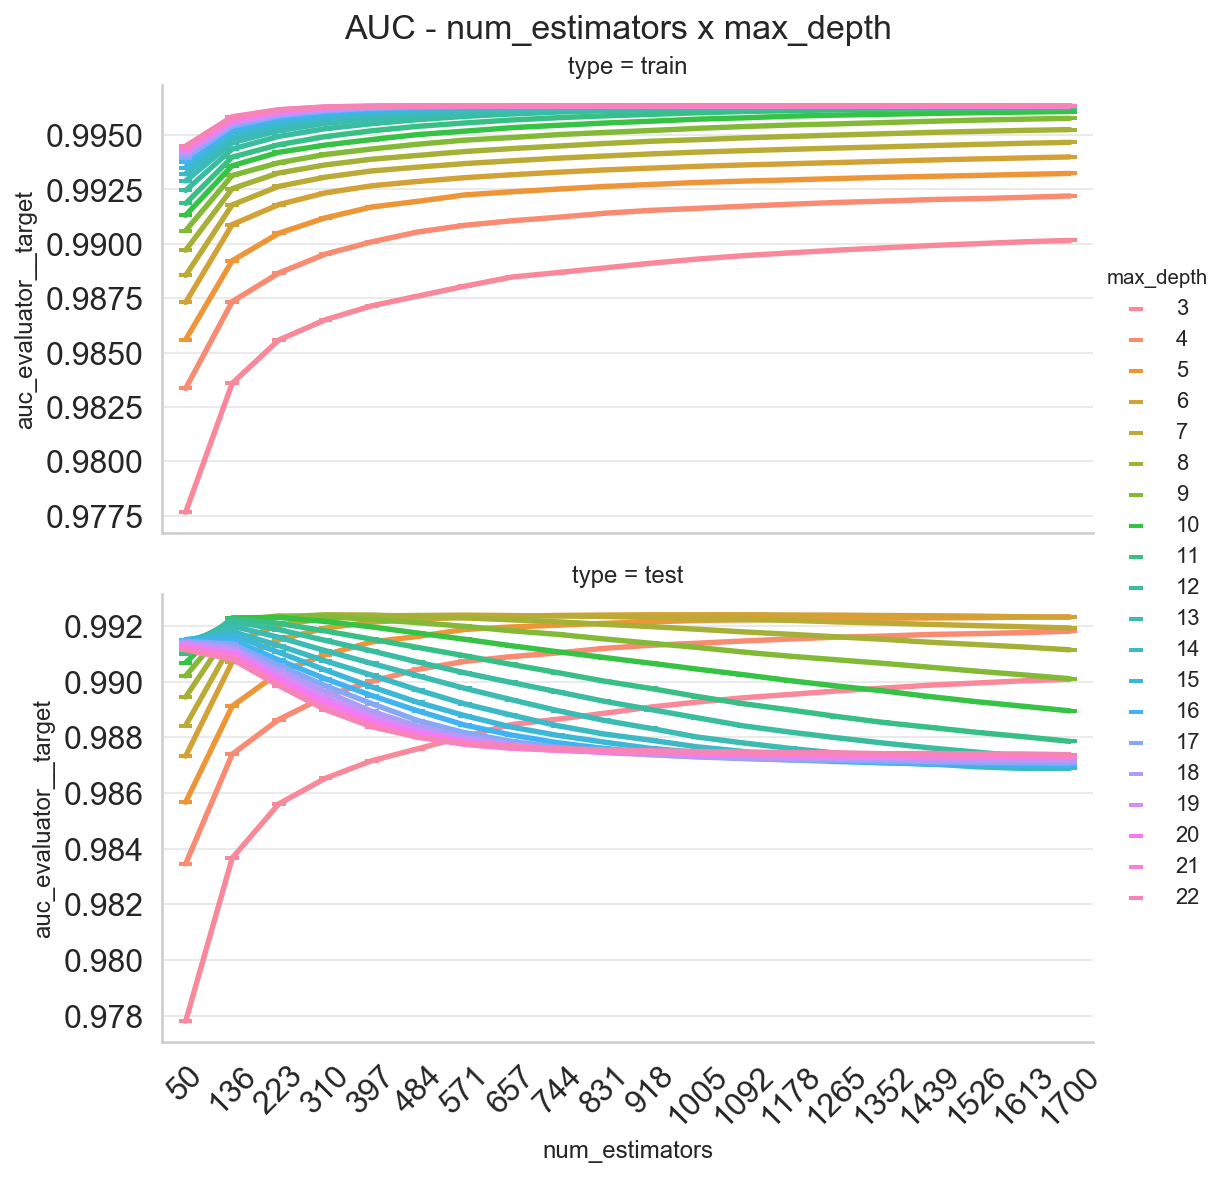
\includegraphics[width=0.8\textwidth]{res-mult1.png} 
    \caption{Pair impact of $MD_i \times NE_i$  on the \textit{BNG(kr-vs-kp)} dataset}
    \label{fig:res-mult1}
\end{figure}

On the other hand, when analyzing \ref{fig:res-mult2} the pair $MD_i \times LR_i$ does not show a clear inversion of the hyperparameters impact: one can only conclude that for \textit{BNG(kr-vs-kp)} lower \textbf{\code{max\_depth}} and high \textbf{\code{learning\_rate}} results in higher AUC (keeping the other hyperparameters the same). This is expected since the learning rate does not have the same ``overfit relationship'' as maximum depth and number of estimators have (explained in \ref{subsec:max-depth}).

\begin{figure}[H]
    \centering
    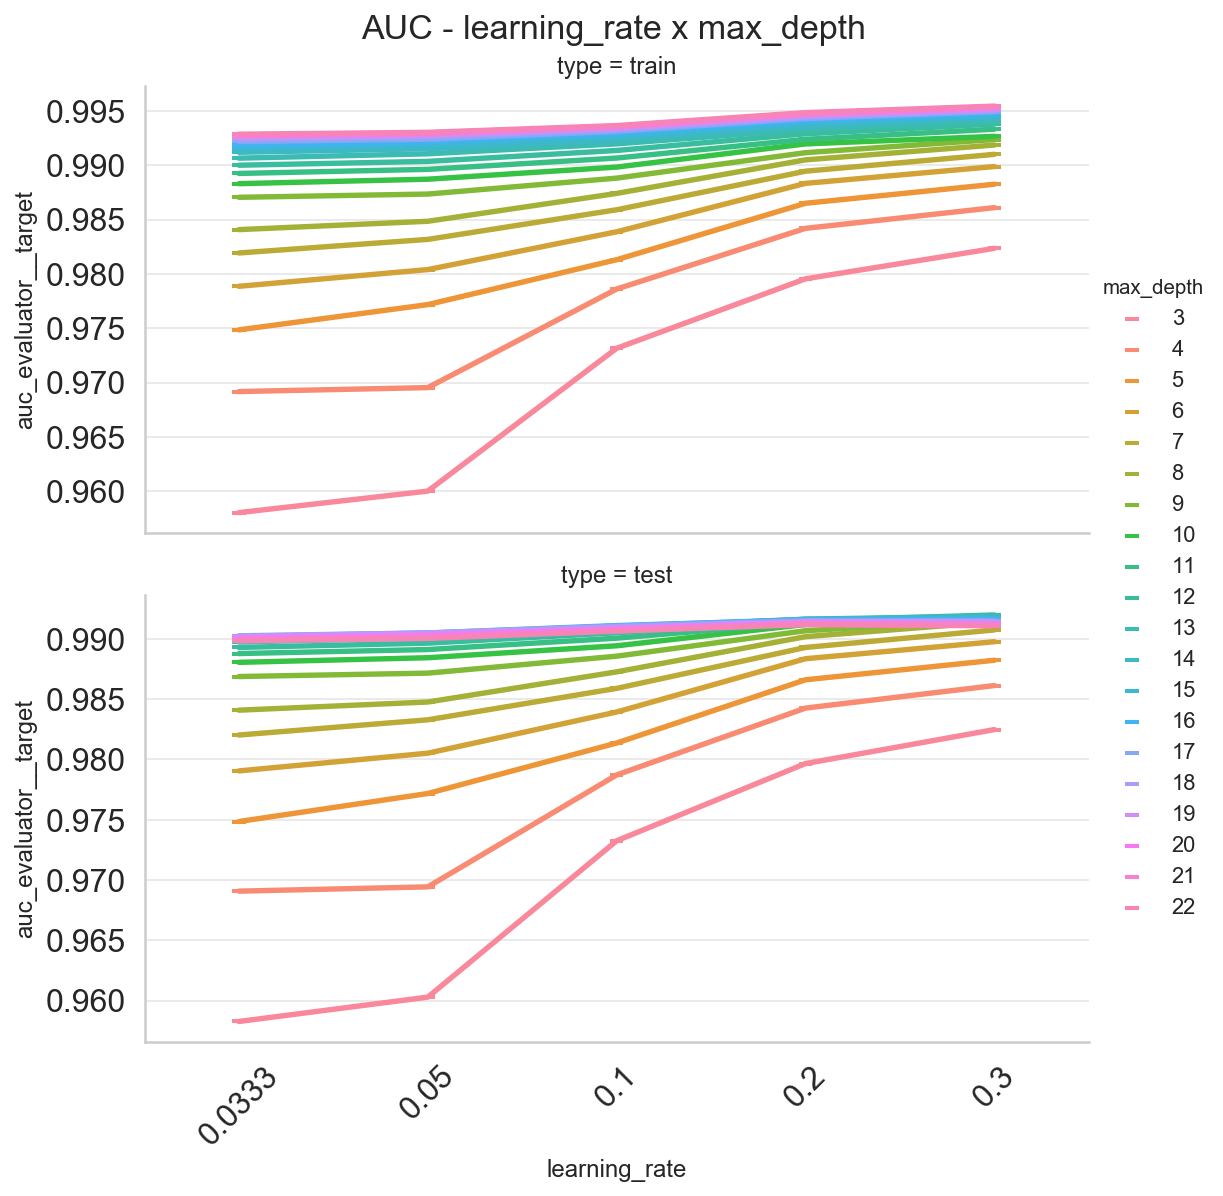
\includegraphics[width=0.8\textwidth]{res-mult2.png}
    \caption{Pair impact of $MD_i \times LR_i$  on the \textit{BNG(kr-vs-kp)} dataset}
    \label{fig:res-mult2}
\end{figure}

\subsection{Hyperparameter Triples Impact}
\label{subsec:triple-impact}

Finally, each dataset is also run using all possible combinations of the studied hyperparameters, i.e. a classical Grid Search run using \code{num\_estimators}, \code{max\_depth} and \code{learning\_rate}. Results of AUC of the triple impact for  \textit{BNG(kr-vs-kp)} can be seen in Figure \ref{fig:res-all1}.

\begin{figure}[H]
    \centering
    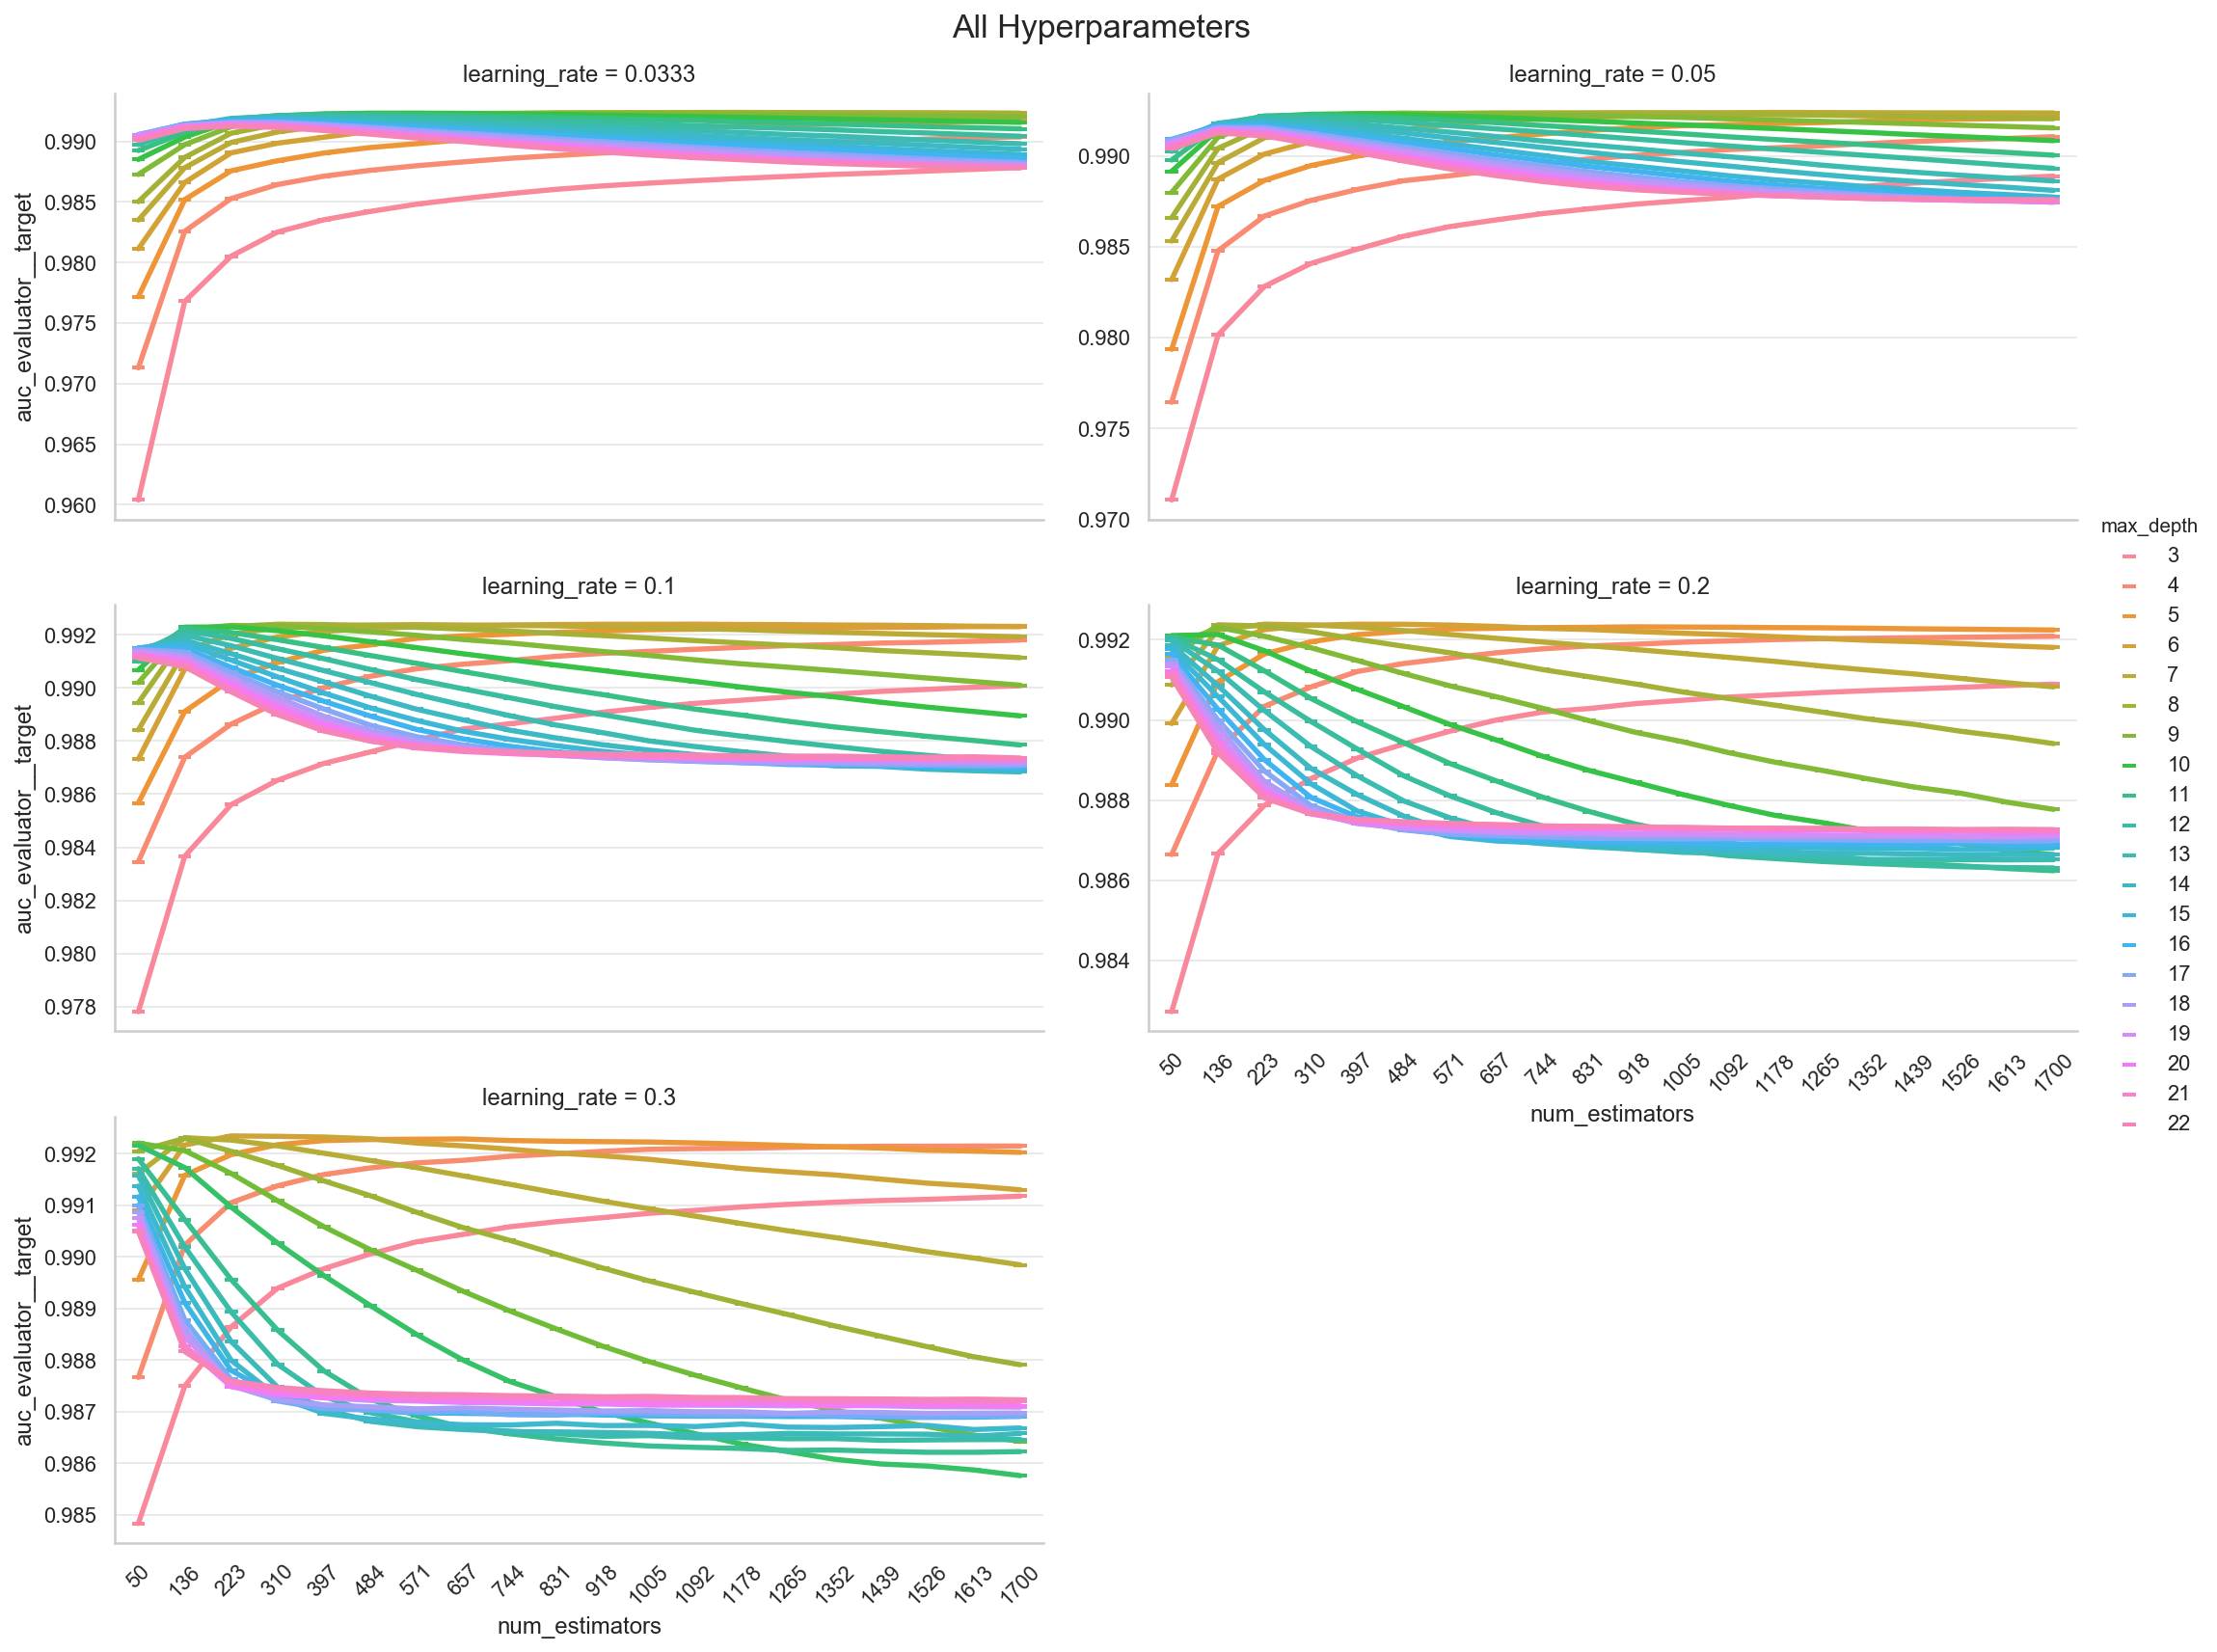
\includegraphics[width=1\textwidth]{res-everything1.png} 
    \caption{Triple impact of hyperparameters on the \textit{BNG(kr-vs-kp)} dataset, showing only \textbf{test} set AUC}
    \label{fig:res-all1}
\end{figure}

One of the inherent difficulties when analyzing these results is due to the high dimensionality of the results: Each experiment has at least three different types of hyperparameters, plus three different metrics for each run. In Subsection \ref{subsec:ordering} this problem will be tackled, with an overview of the statistical techniques and analysis performed to compare and obtain insights into the impact on performance metrics.

%% ------------------------------------------------------------------------- %%
\section{Dataset Aggregation and Clustering}


To tie dataset characteristics to hyperparameters effect in the subsequent analysis, a variety of different measures were calculated in the dataset analysis process, explained in detail in Section \ref{dataset-aggregated-statistics} of Chapter \ref{cap:study-methodology}. When analyzing all datasets' features characteristics, useful insights into the data can be found on it. First, a clear conclusion is that proportion of categorical features in the dataset is much higher than  other types (numeric, Boolean or constants), as demonstrated in Figure \ref{fig:dset-pre1}, and that the most common cardinality is two categories for the categorical features\footnote{These categorical features could be encoded as the \textit{Boolean} feature type, or vice-versa. In the study it was decided that Boolean features are columns which had explicitly \textbf{True} and \textbf{False} as values.}, while few features have high cardinality (Figure \ref{fig:dset-pre2}).

\begin{figure}[H]
    \centering
    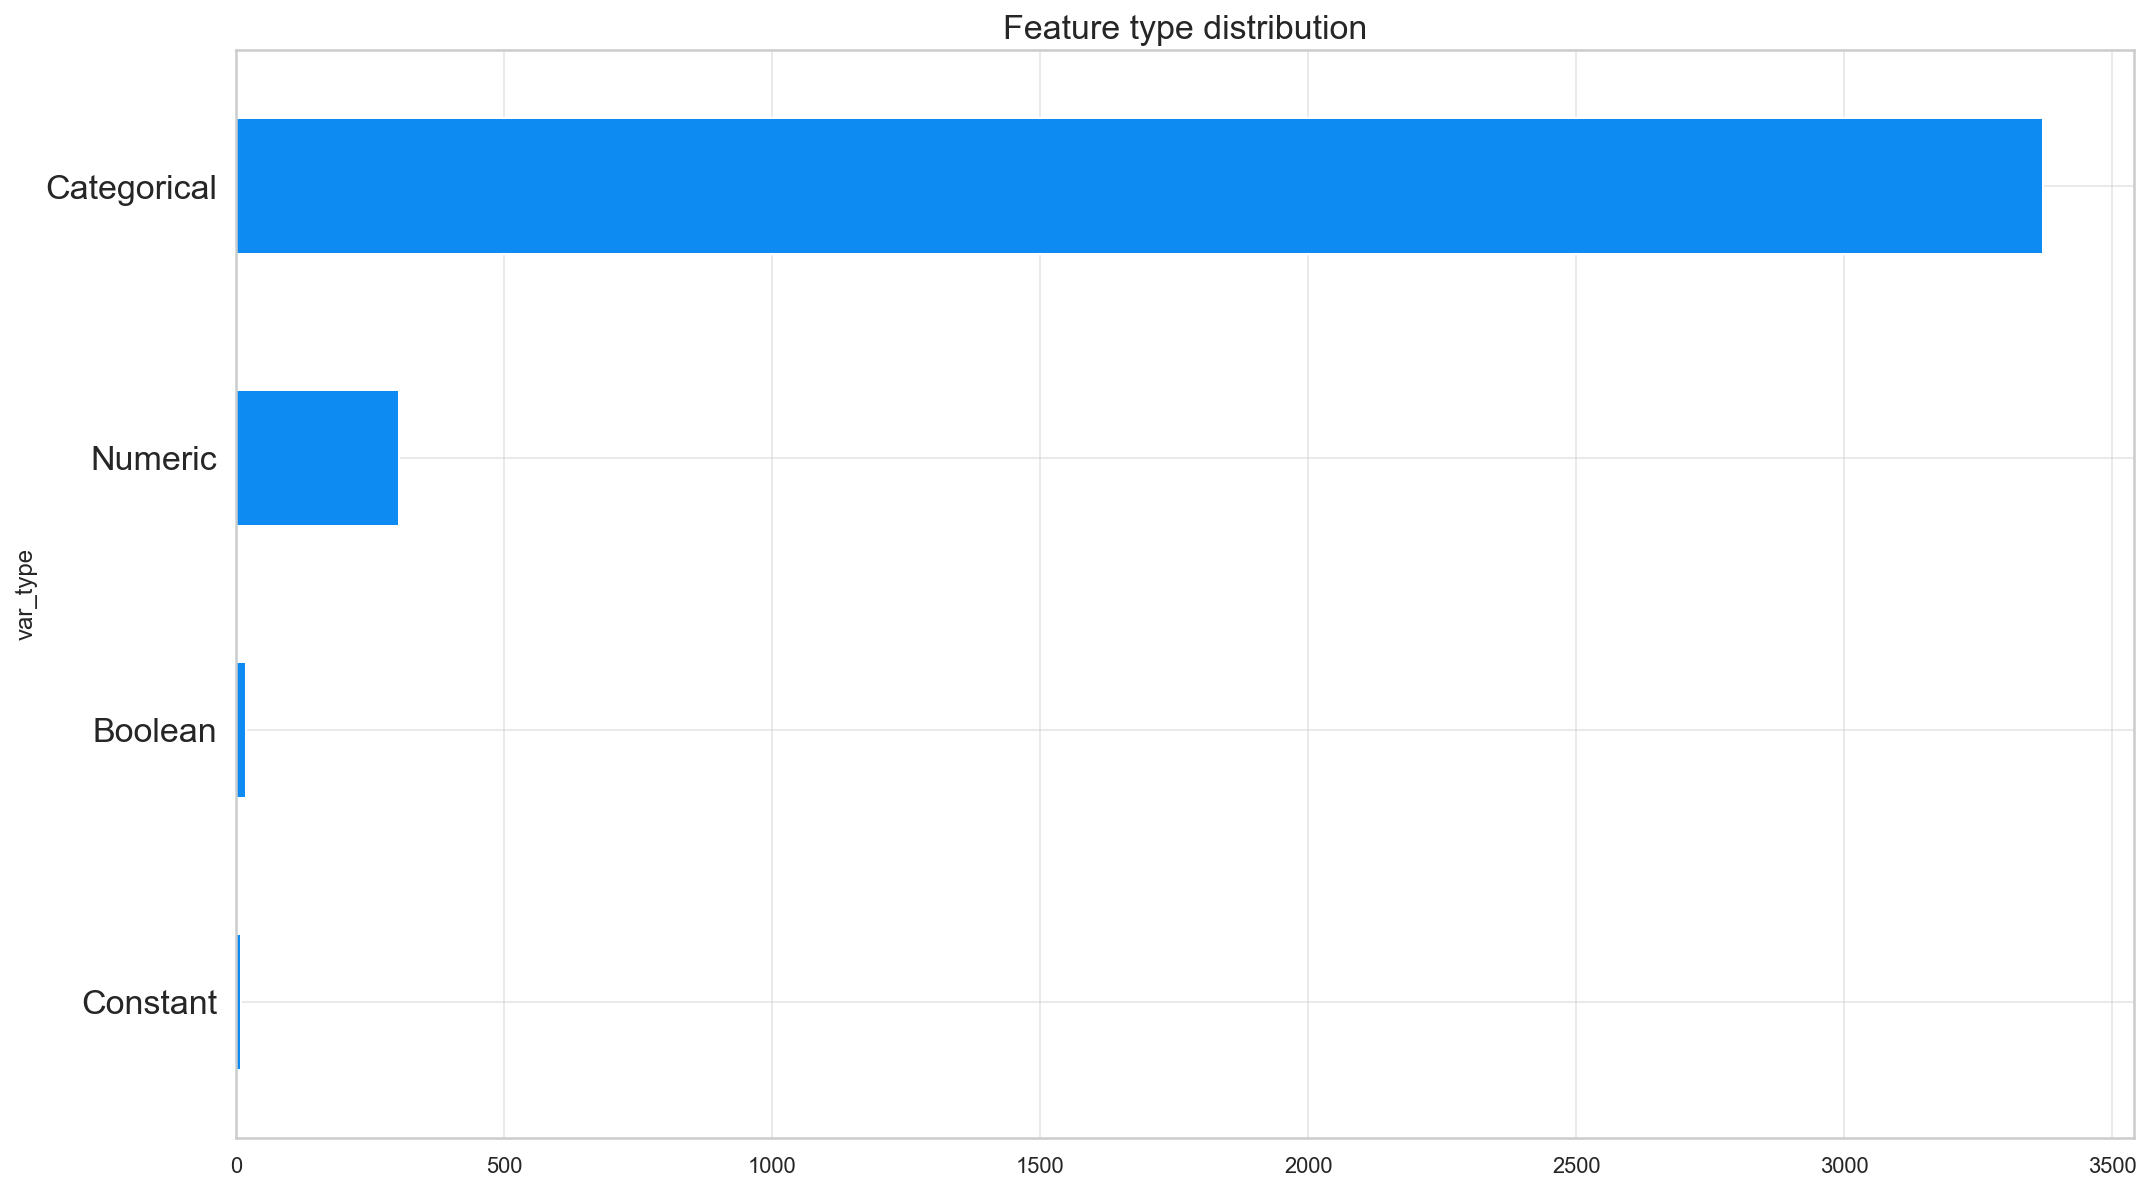
\includegraphics[width=.7\textwidth]{dset-pre1.png} 
    \caption{Feature types of the benchmark datasets}
    \label{fig:dset-pre1}
\end{figure}

\begin{figure}[H]
    \centering
    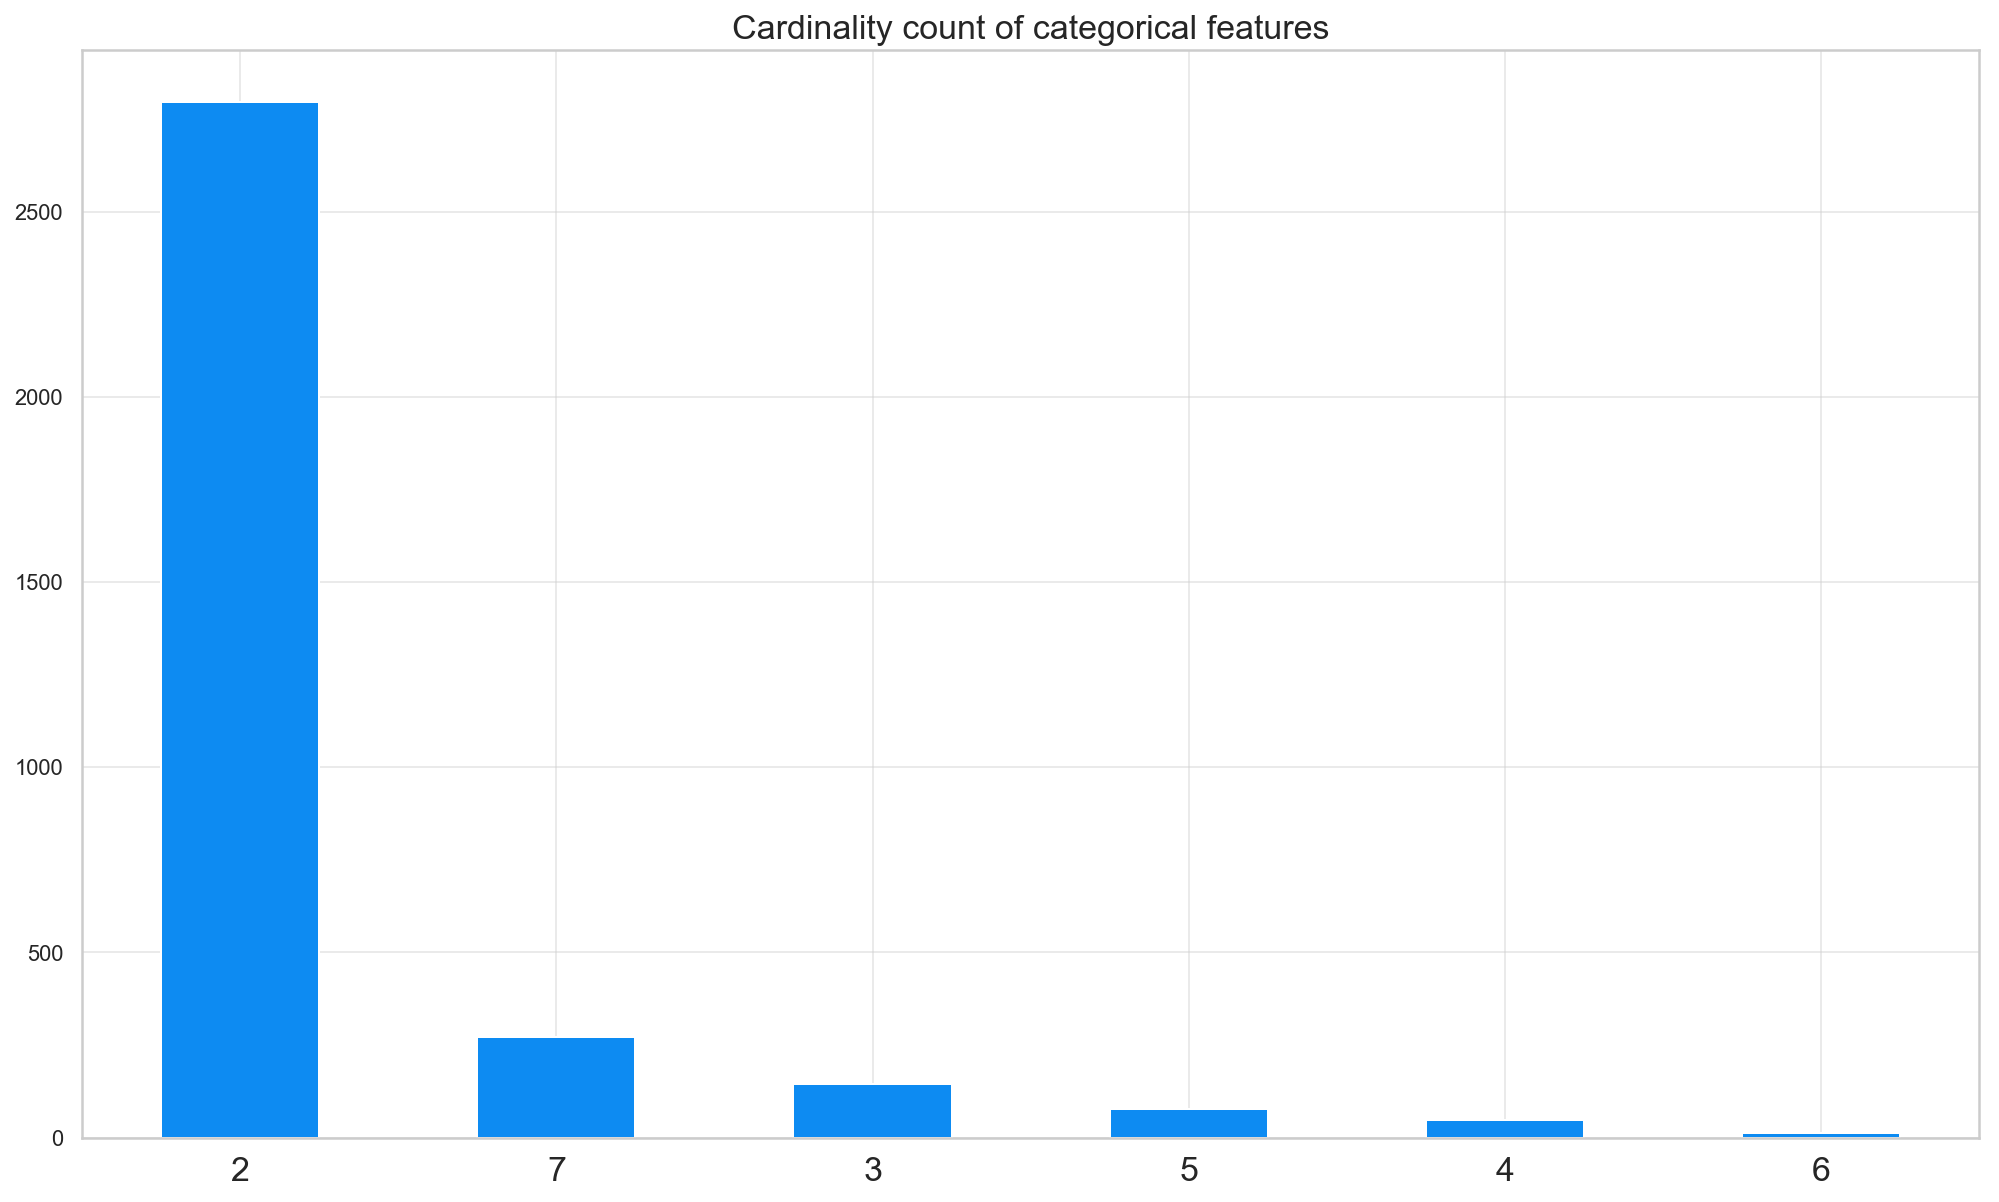
\includegraphics[width=.7\textwidth]{dset-pre2.png} 
    \caption{Cardinality of categorical features of the benchmark datasets}
    \label{fig:dset-pre2}
\end{figure}

With relation to the skewness of the numeric features, most of them have low skewness, with the majority of them having $0$ skewness. This can indicate either that the features themselves do not have innate skewness, or they've been processed different techniques to normalize and remove skewness, like a logarithmic transformation, cubic root transformation, etc. The distribution can be seen in Figure \ref{fig:dset-pre3}.

\begin{figure}[H]
    \centering
    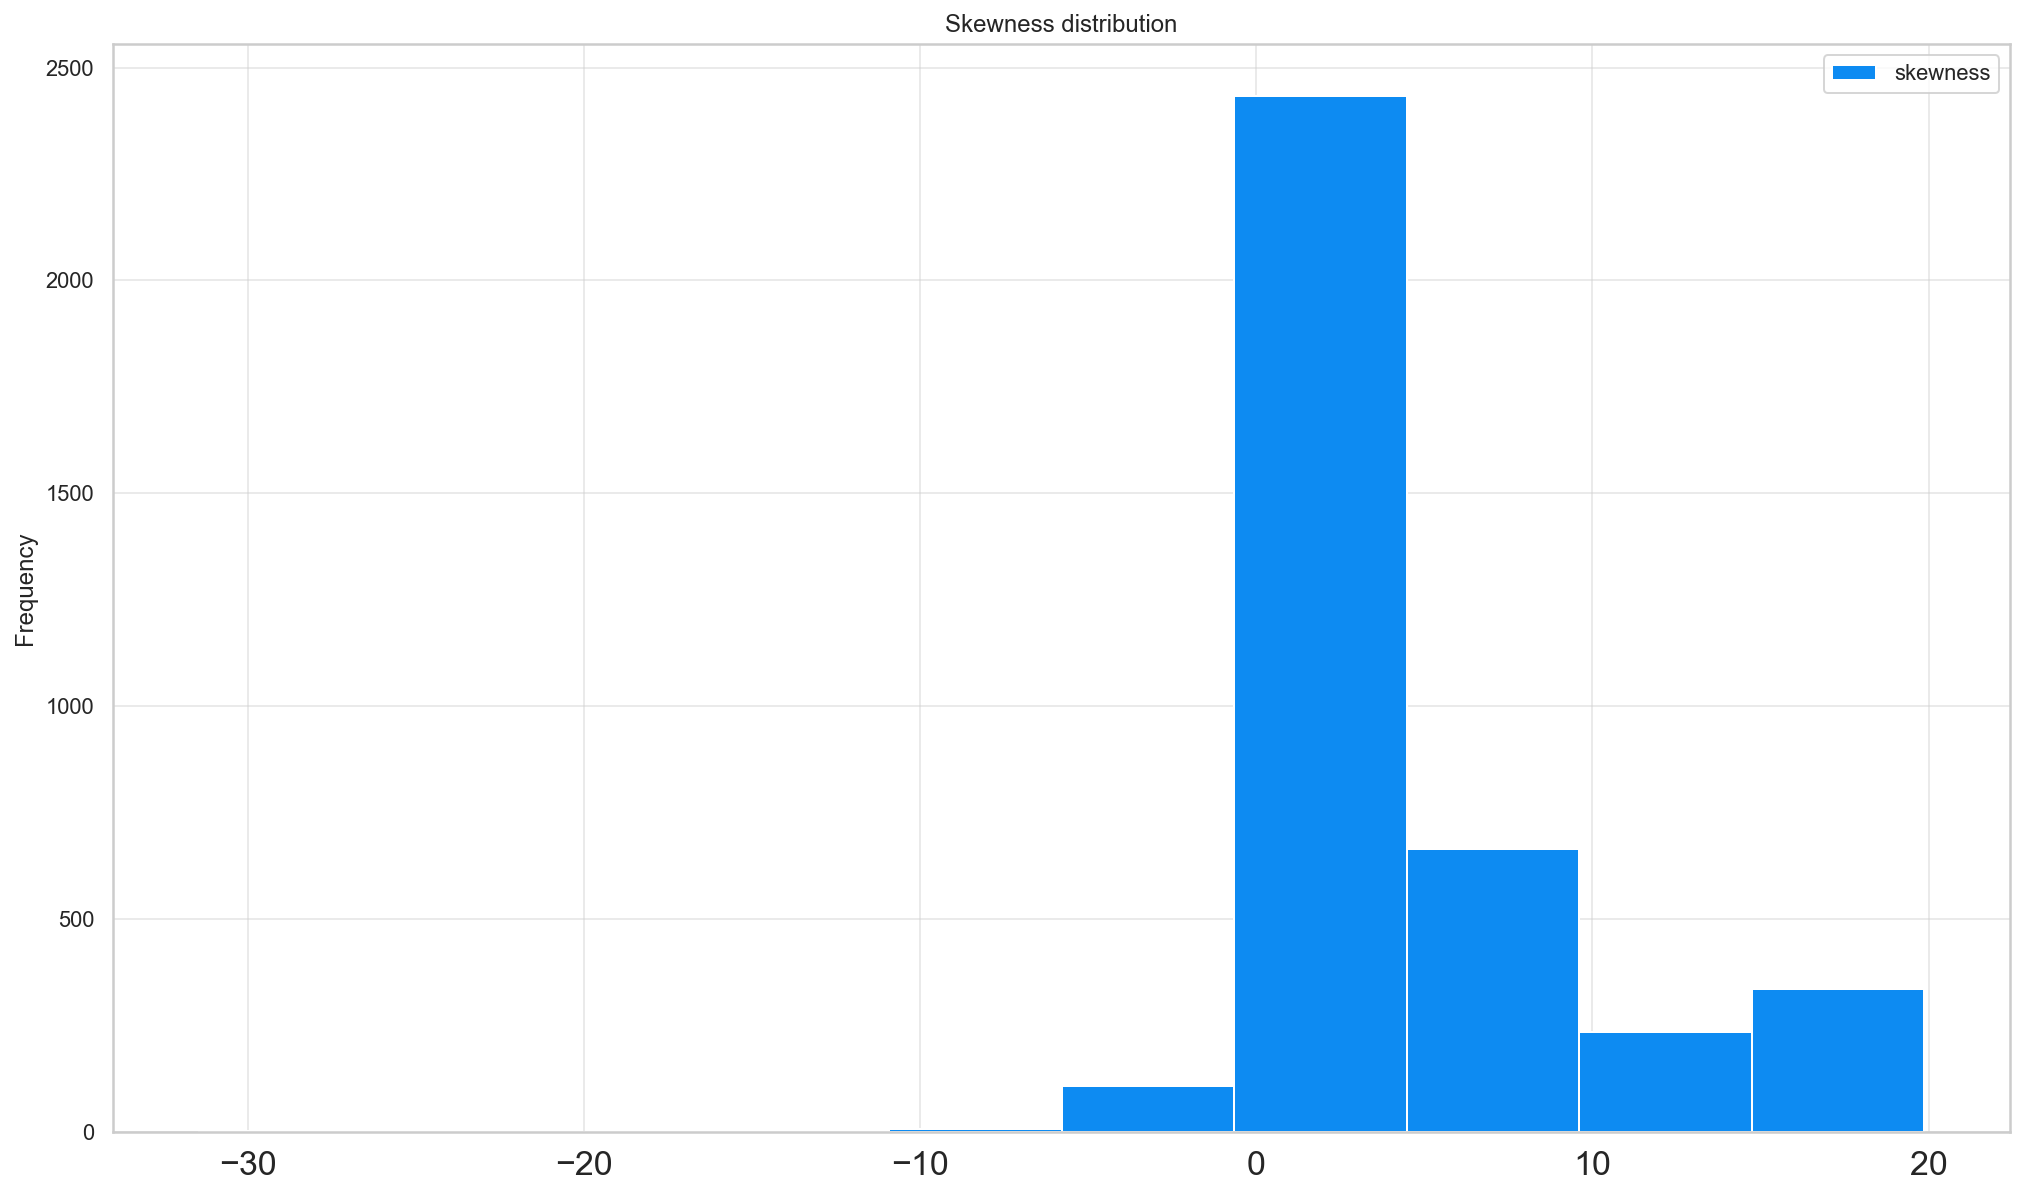
\includegraphics[width=.7\textwidth]{dset-pre3.png}
    \caption{Skewness distribution of the numeric features in the dataset}
    \label{fig:dset-pre3}
\end{figure}

\subsection{Aggregation}
\label{subsec:agg-characteristics}

Since the granularity of the statistics are feature-wise, all datasets were subjected to an aggregation process which combines the feature-wise statistics into \textit{dataset aggregated characteristics}. The objective of this aggregation is to represent each dataset considered in the study into a point in a high dimensional space, which gives power to perform a multitude of transformations and comparisons, and in the case of this study, a clustering by the similarity of the datasets according to these aggregated values. For each dataset, the following aggregations are made:

\begin{itemize}
    \item \textbf{\code{num\_rows}}: Number of rows in the dataset, i.e. the number of instances of $D_i$;
    \item \textbf{\code{num\_features}}: Number of features in the dataset;
    \item \textbf{\code{mean\_skewness}}: $0$ if there is no numeric features in the dataset, otherwise the mean of the skewness of the numeric features;
    \item \textbf{\code{mean\_variance}}: The mean of the \textit{variance} of categorical features, where the variance concept is the one described at Section \ref{dataset-aggregated-statistics};
    \item \textbf{\code{num\_categorical}}: How many categorical features the dataset has;
    \item \textbf{\code{sum\_cardinality\_over\_categorical}}: Let $K$ be the set of categorical features of the dataset, and $Cardinality_K$ the sum of the cardinality of all $k\in K$. Then, this aggregation is defined as $\frac{Cardinality_K}{|K| + 1}$, which is simply the "\textit{mean}" of cardinality in the dataset. The $+1$ is to avoid error with datasets which do not have categorical features;
    \item \textbf{\code{categorical\_ratio}}: Proportion of categorical features in the dataset;
    \item \textbf{\code{numeric\_ratio}}: Proportion of numeric features;
    \item \textbf{\code{boolean\_ratio}}: Proportion of Boolean features;
    \item \textbf{\code{constant\_ratio}}: Proportion of constant features.
\end{itemize}


After this transformation, each dataset $D_i$ is now represented by a $\mathcal{P}_i \in \mathbb{R}^{10}$ where each component of the multidimensional point represents one of the aggregated characteristics calculated above. To visualize these multidimensional points, a t-SNE projection (dimensionality reduction technique, more details in \cite{maaten2008visualizing}) on two dimensions is shown in Figure \ref{fig:tsne-1}.

\begin{figure}[!h]
    \centering
    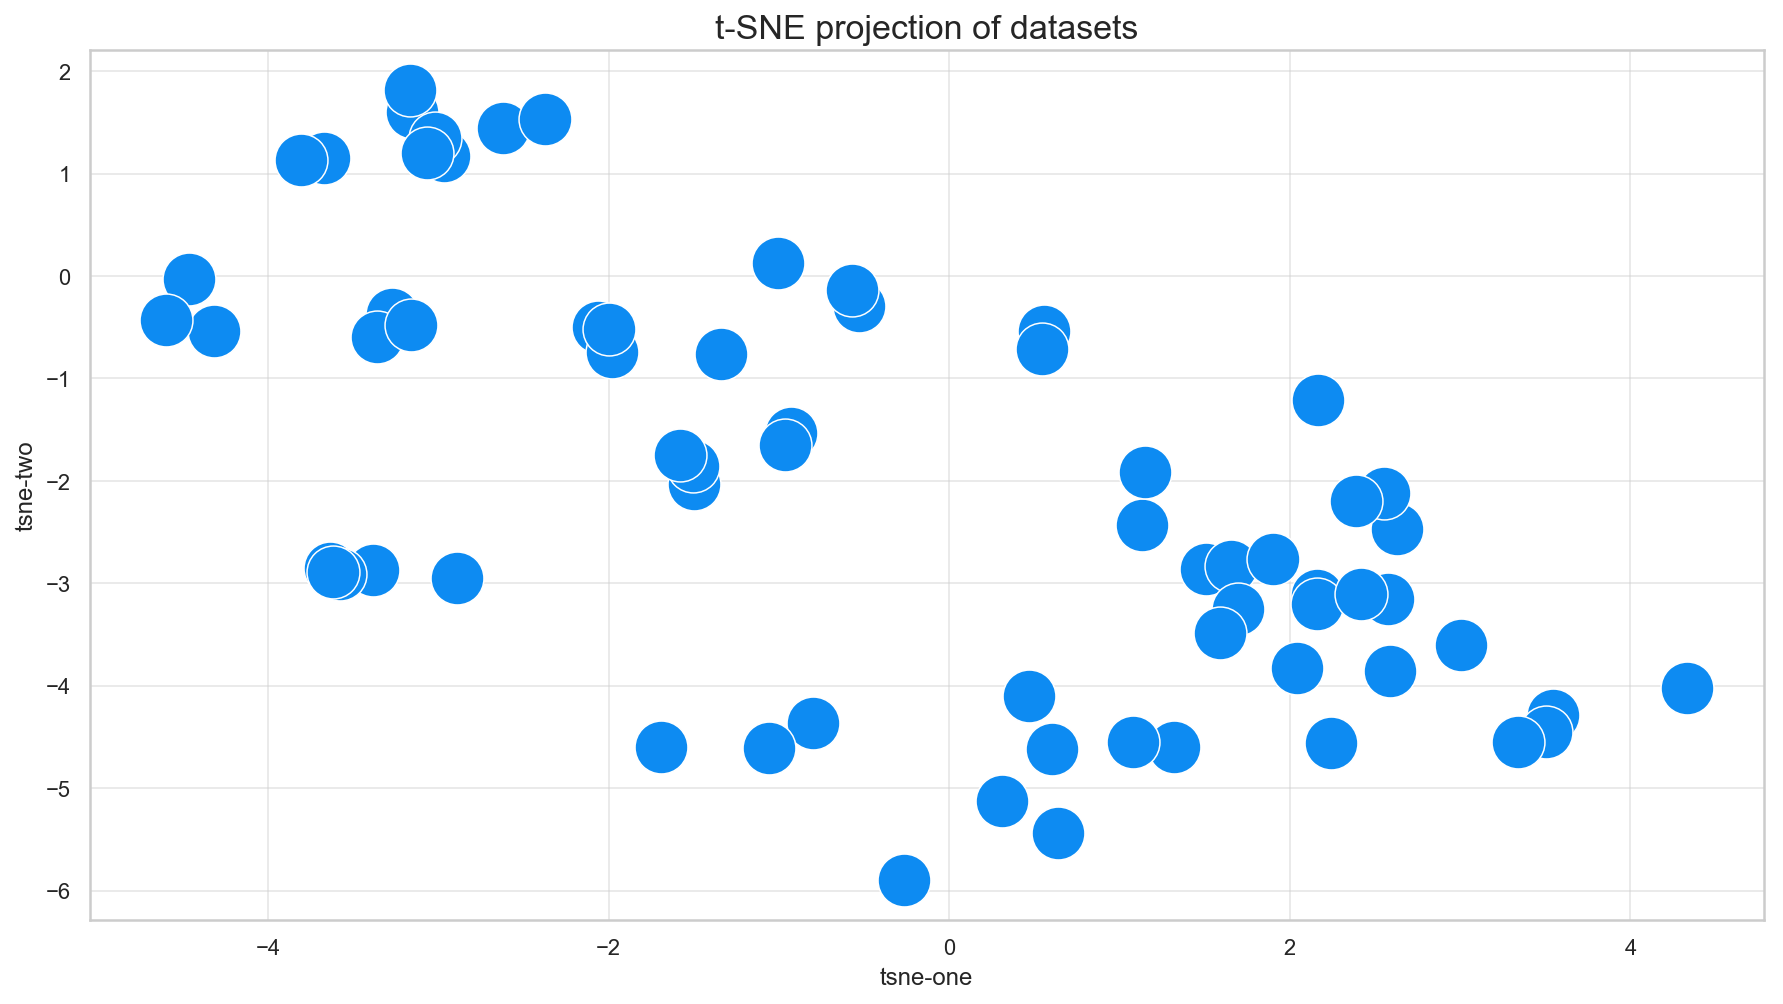
\includegraphics[width=1\textwidth]{tsne1.png}
    \caption{t-SNE projection of all $\mathcal{P}_i$}
    \label{fig:tsne-1}
\end{figure}

The aggregated characteristics were designed in a way to encompass both the proportion of feature types in the dataset and the absolute size of the dataset. The \code{*ratio} aggregations are done to compare multiple datasets regardless of the absolute numeric value of features it has but on the ratio of the feature types. On the other hand, the absolute features like \code{num\_rows} captures the absolute size of the data. For example, a simple analysis using \code{num\_rows}, \code{num\_features} and \code{categorical\_ratio} could yield interesting insights and a way to bundle similar datasets together based on the proportion of categorical features, controlling for both the number of data points and the number of features. 

Finally, there is also an explicit emphasis on characteristics regarding numeric and categorical features, which are of interest in this study (more information about the premisses about it on Section \ref{dataset-aggregated-statistics} of Chapter \ref{cap:study-methodology}). The mean of skewness aggregation can be used to control (in the experimental design sense) for datasets with a similar distribution of skewed or not numerical features, while the mean of variance, the number of categorical features and the "\textit{mean}" of cardinality describes important information regarding the categorical aspect of the dataset.  

\subsection{Clustering Strategy}
\label{subsec:clustering-strat}
To analyze all experiments based on similar dataset characteristics, the decided approach was to perform a simple clustering technique, instead of manually selecting which datasets are similar by looking at the aggregated characteristics by hand. Using the aggregated characteristics explained in the last section, a clustering approach on the points $\mathcal{P}_i$ generates clusters based on those characteristics.

\begin{figure}[!h]
    \centering
    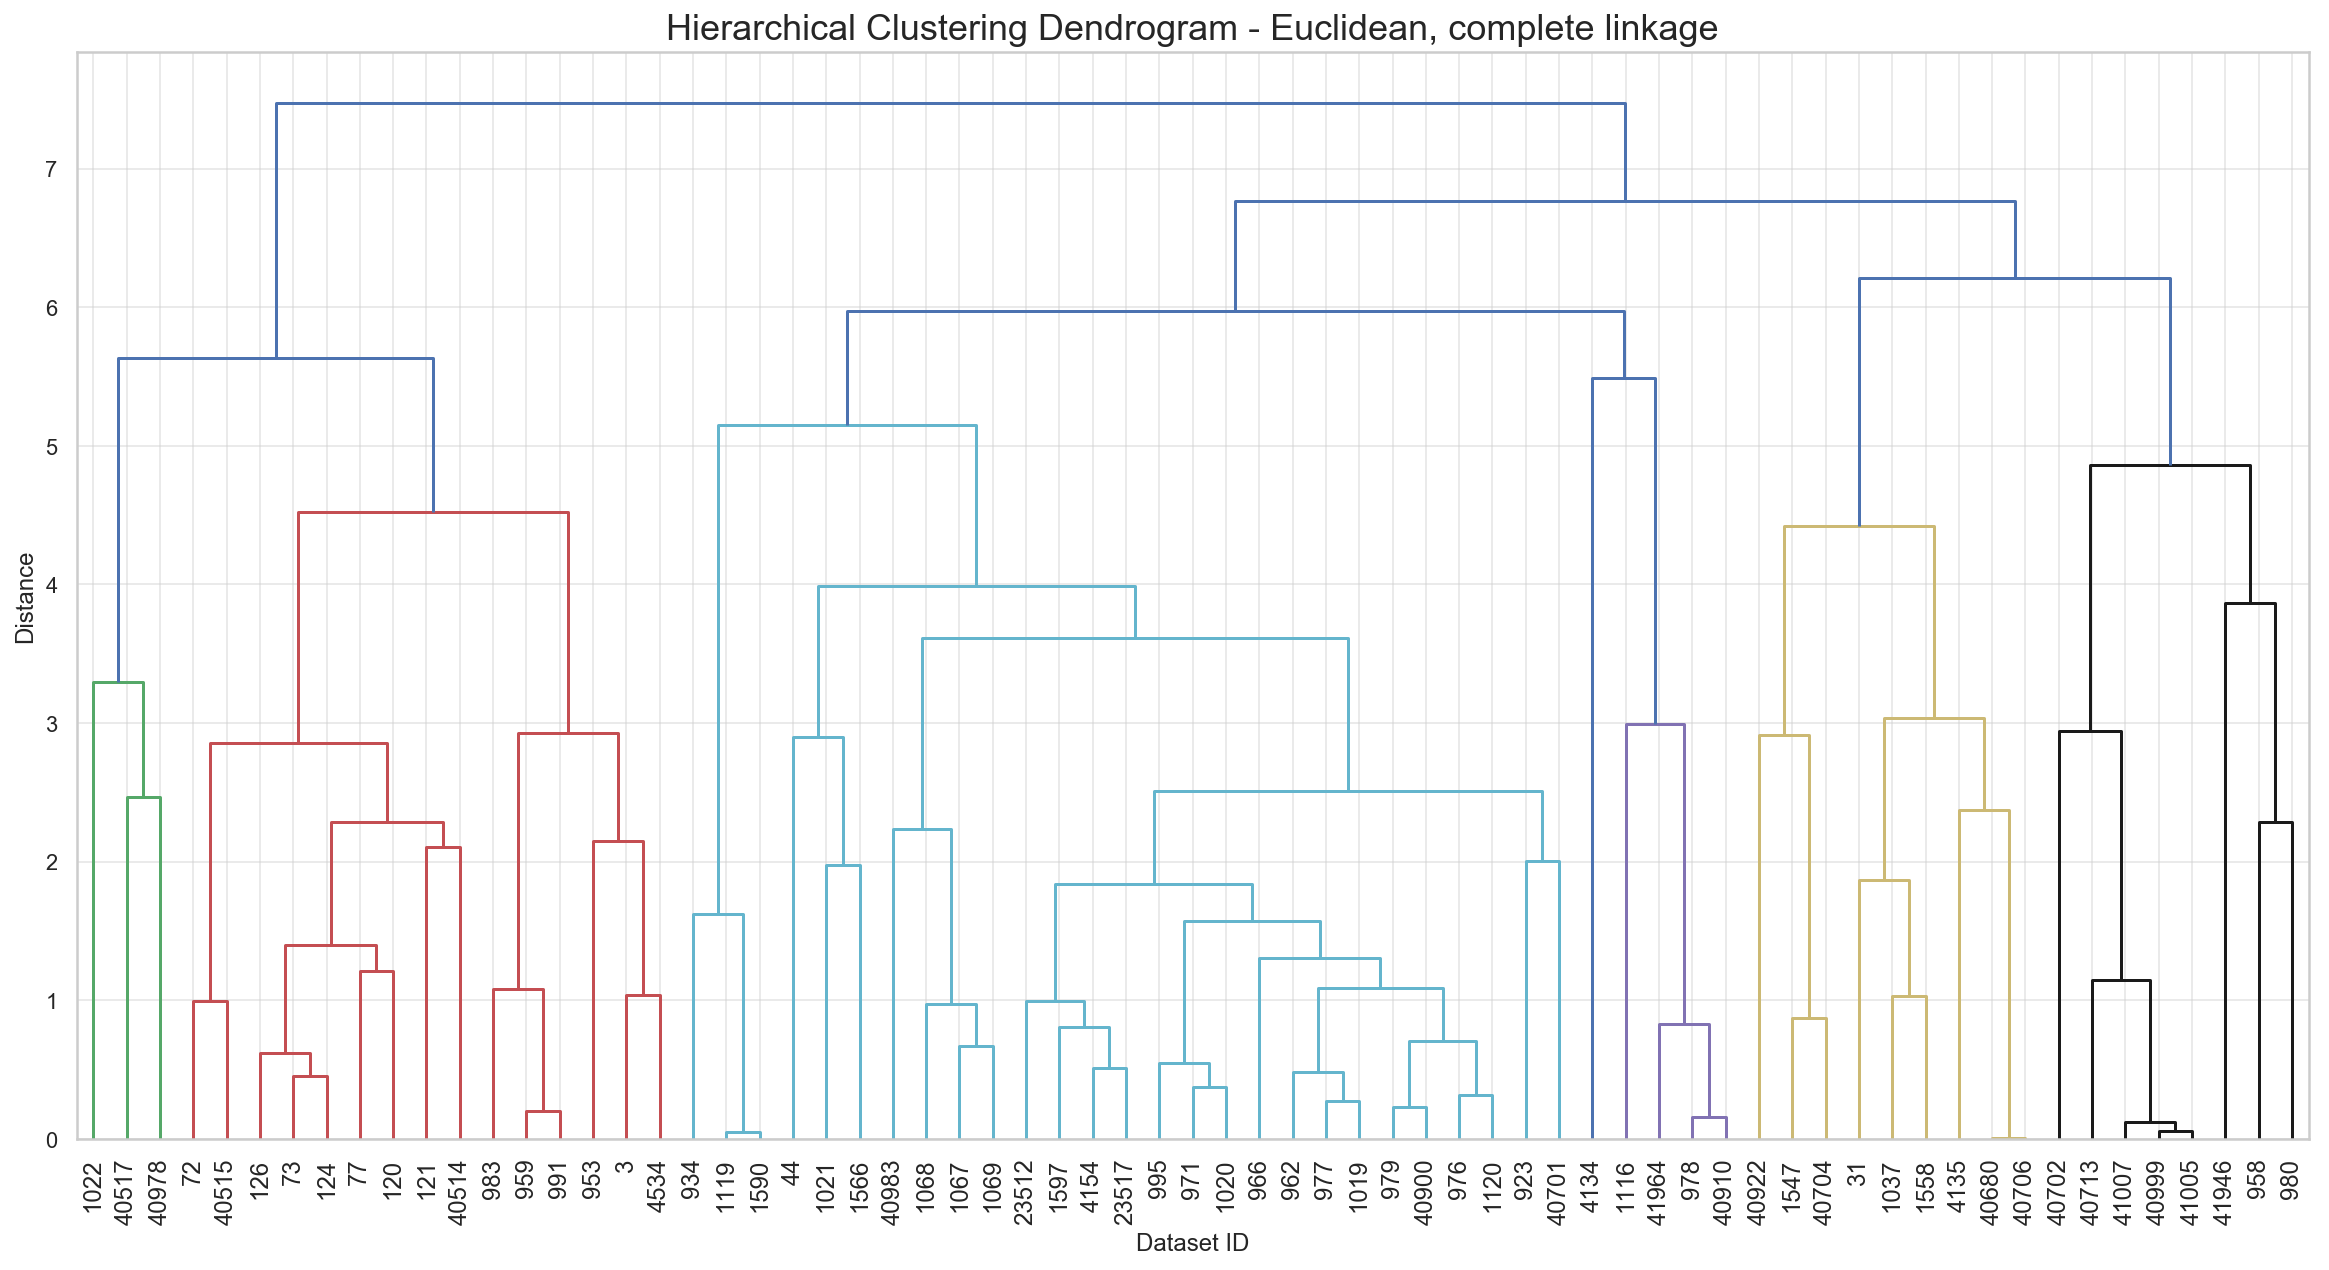
\includegraphics[width=1\textwidth]{dendrogram.png}
    \caption{Dendrogram of the old clustering method}
    \label{fig:dendrogram}
\end{figure}

After some initial experimentation, the chosen clustering approach was to use the well known K-means algorithm, with $k=6$ clusters. K-means is a very simple algorithm that reduces the data to \textit{centroids}, and resulted in reasonable clusters for this study. The other tested technique was to use agglomerative hierarchical clustering and choose the number of clusters by analyzing the resulting dendrogram (the dendrogram for the hierarchical clustering is shown in Figure \ref{fig:dendrogram}). However, this technique generated an uneven number of datasets in each cluster, more than K-means, so the K-means was chosen. It is important to note that the algorithms and the number of clusters chosen here can highly impact the subsequent analysis of the experiment results. The objective is not to create a generic analysis that could work with any possible dataset, but to actually measure the impact of hyperparameters into specific clusters which follow a similar distribution of the aggregated characteristics.

After the K-means procedure, the assigned clusters can be seen in the t-SNE projection in Figure \ref{fig:tsne-2}, where each color represents a different cluster. Even though the number of $\mathcal{P}_i$ in each cluster is not uniform, the clustering assignment is more intuitive, albeit in reduced dimensionality. As an observation note, the two t-SNE projections (Figure \ref{fig:tsne-1} and  \ref{fig:tsne-2}) are different because the embeddings in low dimension change when new data is introduced. In this case, the centroids were also added to the dataset before using t-SNE.

\begin{figure}[h!]
    \centering
    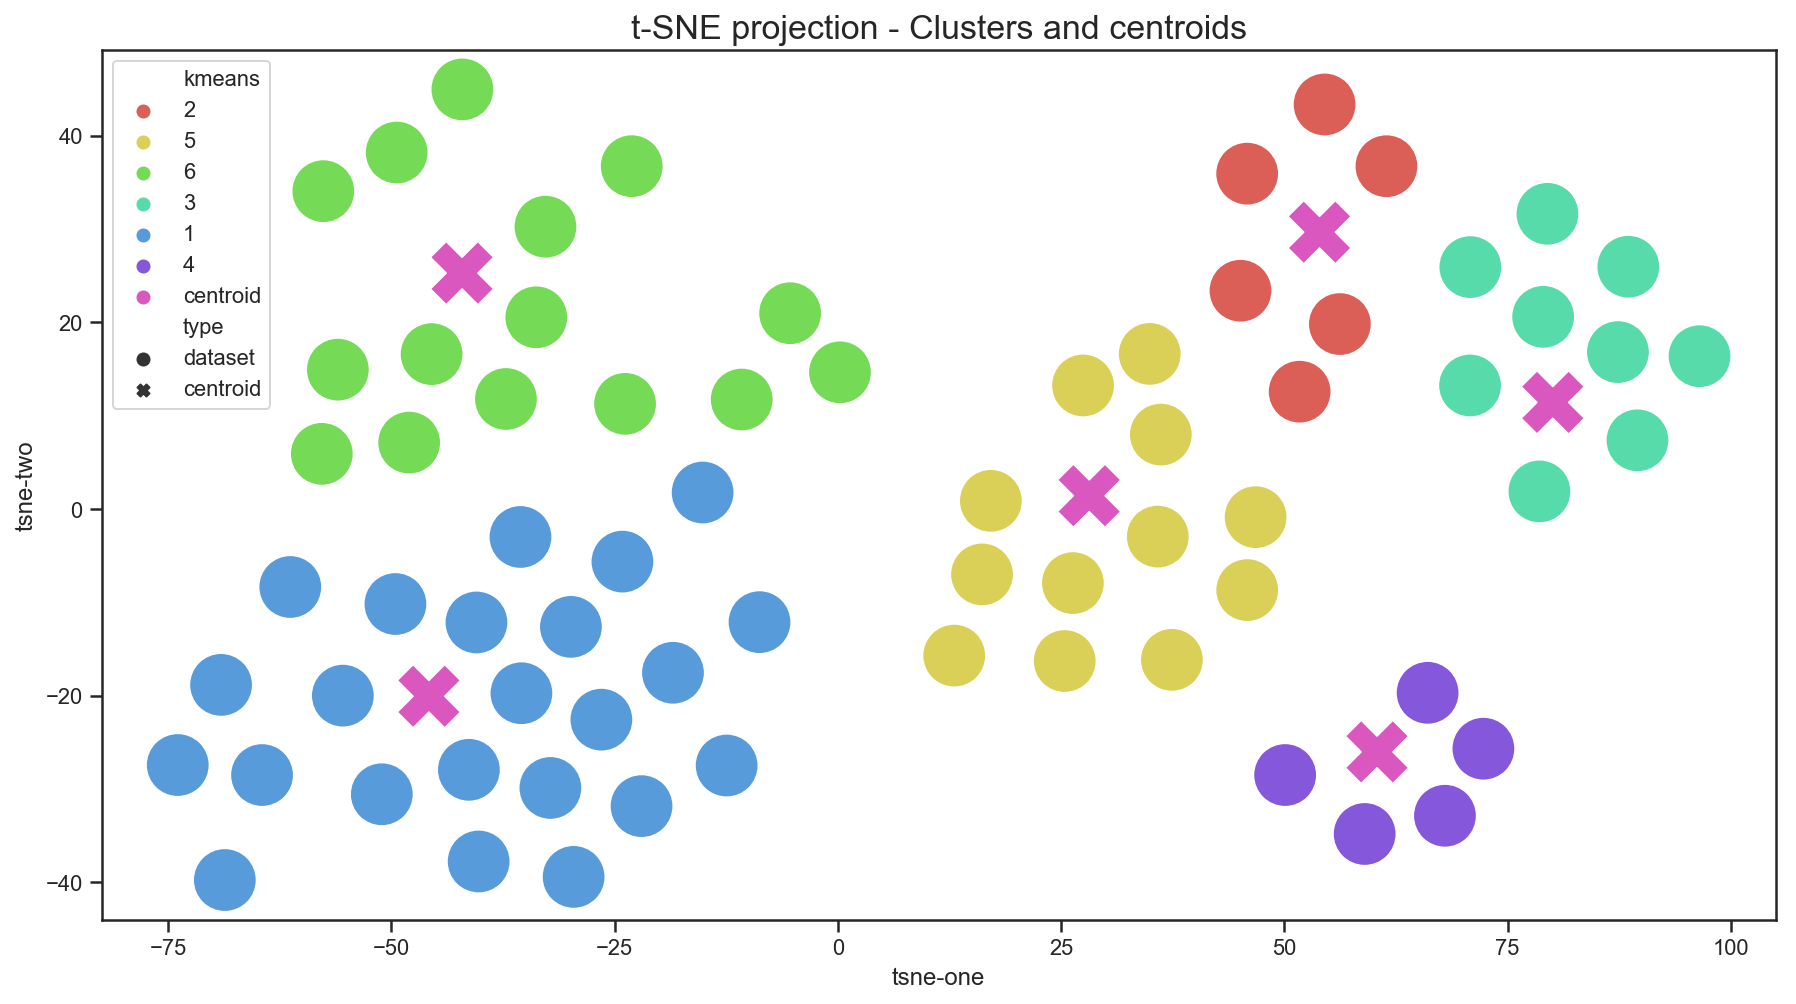
\includegraphics[width=1\textwidth]{tsne2.png}
    \caption{t-SNE projection with the assigned clusters and the centroids}
    \label{fig:tsne-2}
\end{figure}

To understand better the behavior and general characteristics of each dataset of clusters, a superficial manual analysis of the datasets in each cluster is performed. As an example, the names of the datasets from Cluster 2 and 3 are described in Table \ref{table:1}. From the superficial analysis of the content of each dataset, one can see that most of the datasets in Cluster 2 have a high number of categorical features, while datasets in Cluster 3 are all synthetically augmented, i.e. Bayesian Network Generated (\textit{BNG}) and have a very high number of rows.

\begin{table}[h!] 
    \centering
    \begin{tabular}{||c c||} 
     \hline
     Cluster 2 & Cluster 3 \\ [0.5ex] 
     \hline\hline
     \textit{kr-vs-kp} & \textit{BNG(kr-vs-kp)} \\
     \textit{splice} & \textit{BNG(labor,nominal,1000000)} \\
     \textit{mfeat-pixel} & \textit{BNG(breast-cancer,nominal,1000000)} \\
     \textit{PhishingWebsites} & \textit{BNG(mushroom)} \\
     \textit{20\_newsgroups.drift} & \textit{BNG(colic.ORIG,nominal,1000000)} \\
     \textit{Internet-Advertisements} & \textit{BNG(credit-a,nominal,1000000)} \\
     & \textit{BNG(credit-g,nominal,1000000)} \\
     & \textit{BNG(credit-g)} \\[1ex] 
     \hline
    \end{tabular}
    \caption{Datasets from Cluster 2 and Cluster 3}
    \label{table:1}
\end{table}

Using ridgeline plots is another way to understand the meaning of each cluster. By calculating the distribution of the aggregated characteristics over each cluster and plotting them on the same scale against each other, it is possible to evaluate if the clustering makes sense. In total there are $10$ ridgeline plots, one for each aggregated characteristic. Here two of them are illustrated: In Figure \ref{fig:joyplot-1} and Figure \ref{fig:joyplot-2} the ridgeline plots for \code{categorical\_ratio} and \code{mean\_skewness} can be seen. It is easy to see that Cluster 2 datasets have a very high categorical ratio with very little variance, i.e. almost all of the datasets in this cluster contains a high proportion of categorical features. Clusters 1 and 6 have the lowest proportion of categorical features amongst all Clusters. Another conclusion is that Cluster 6 contains more skewed features, as its distribution is skewed towards high \code{mean\_skewness} values.

All the remaining ridgeline plots are available on the appendix \ref{ape:joyplots}.

\begin{figure}[H]
    \centering
    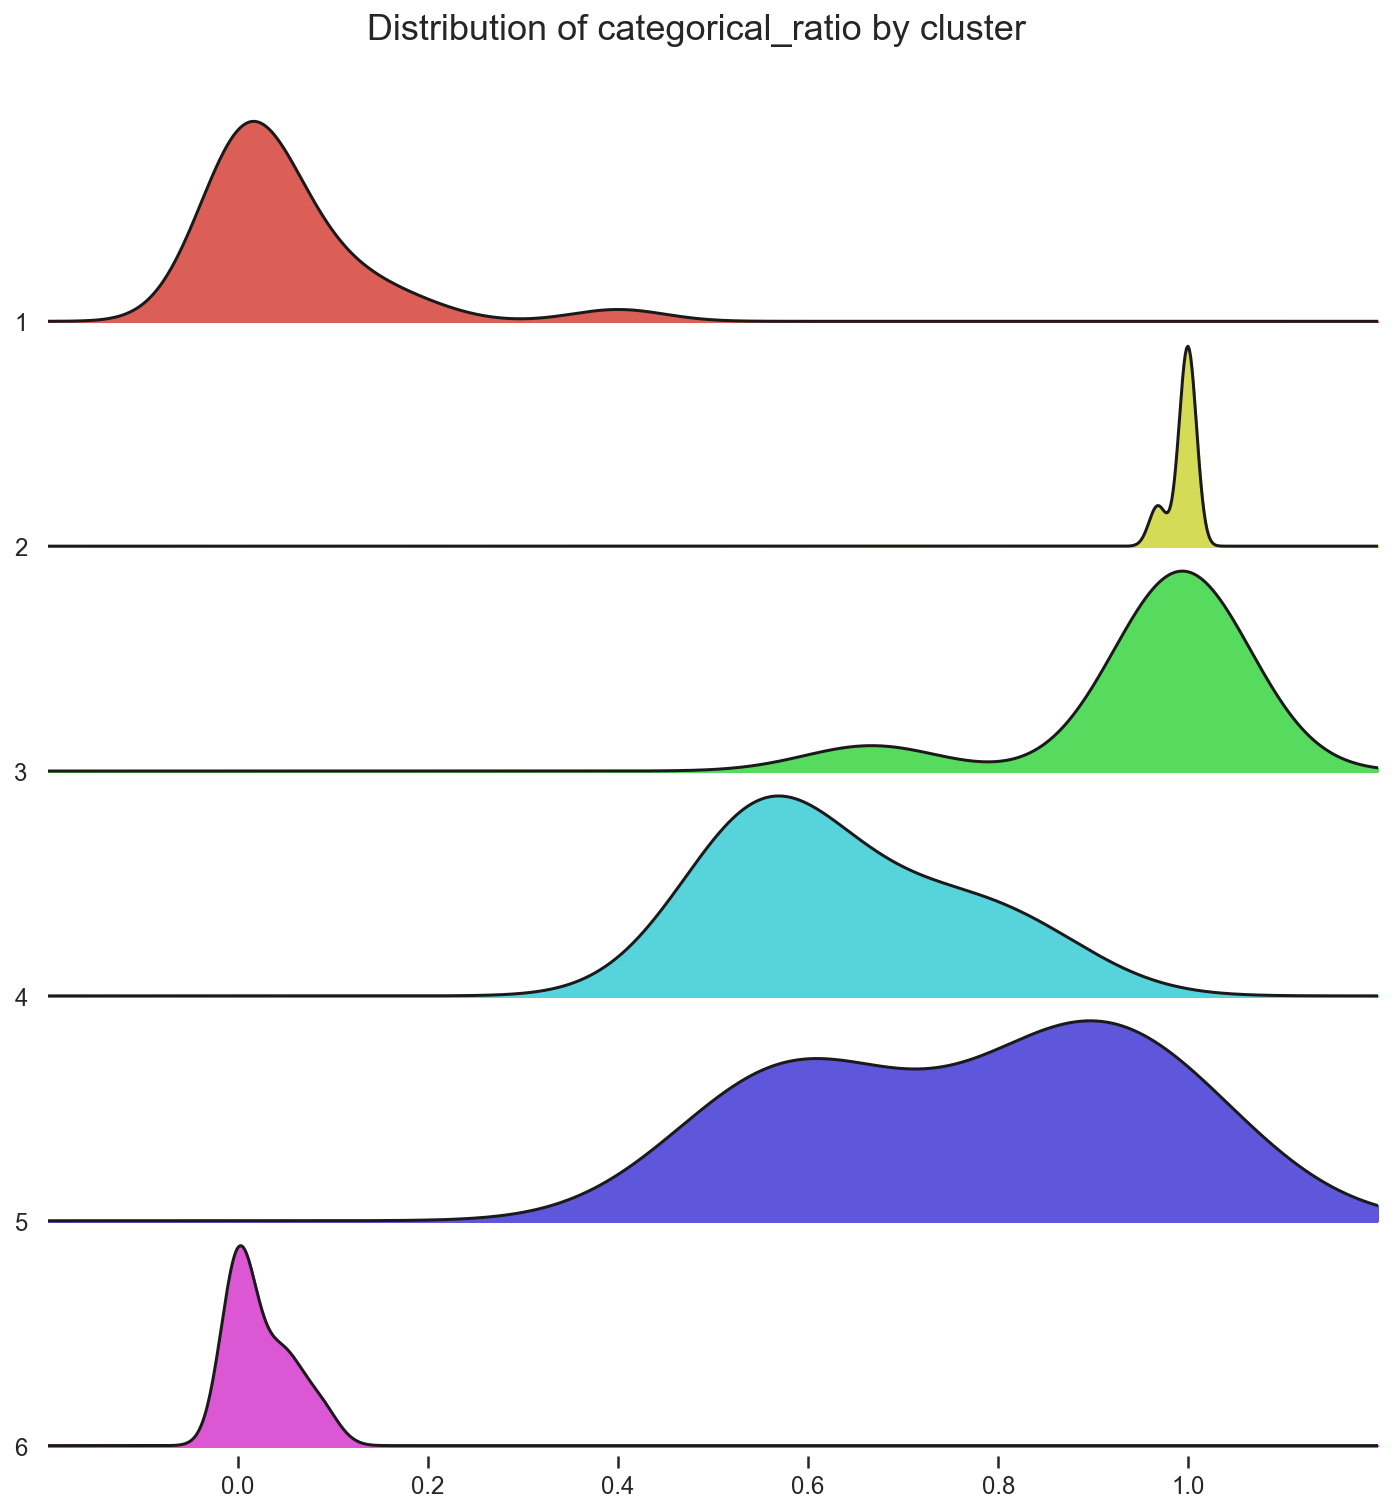
\includegraphics[width=.7\textwidth, height=.6\textwidth]{joyplot1.png}
    \caption{Ridgeline plot of \code{categorical\_ratio}. Clusters are represented by different colors}
    \label{fig:joyplot-1}
\end{figure}

\begin{figure}[H]
    \centering
    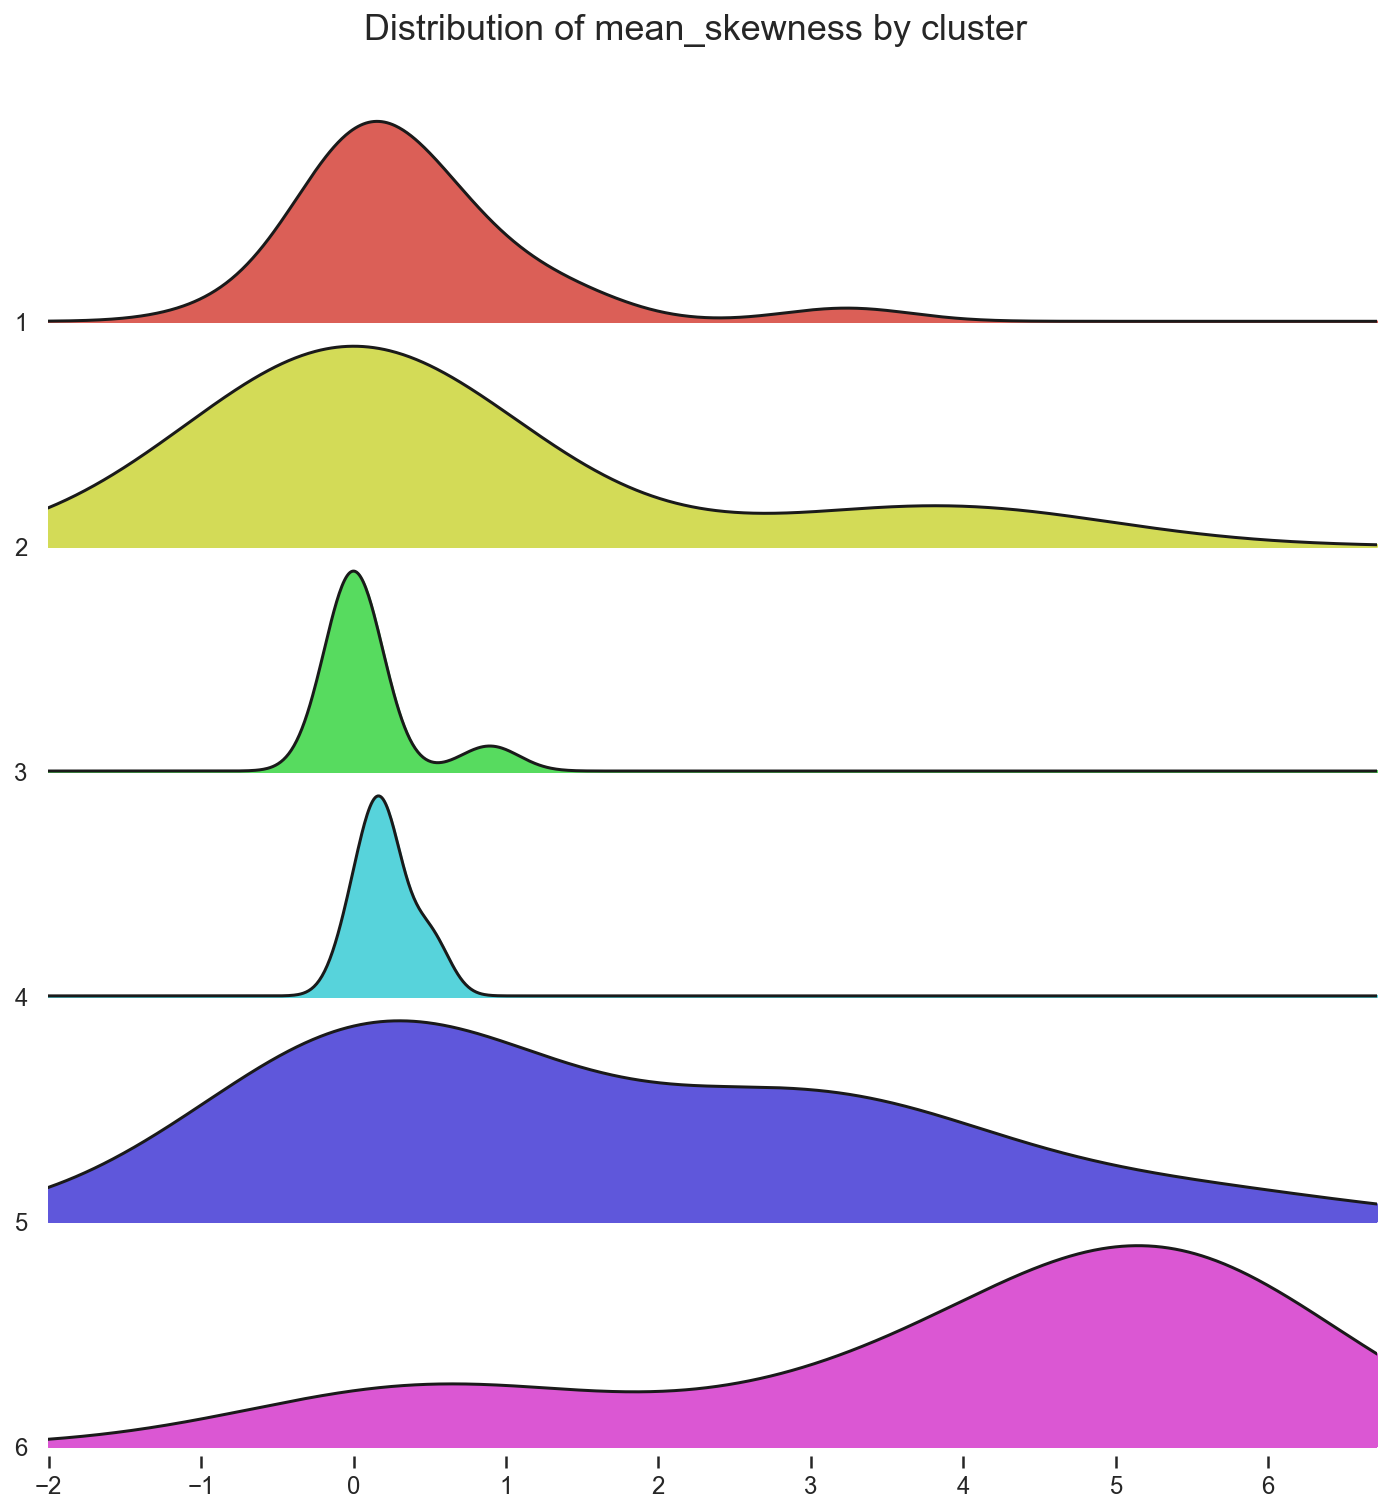
\includegraphics[width=.7\textwidth, height=.6\textwidth]{joyplot2.png}
    \caption{Ridgeline plot of \code{mean\_skewness}. Clusters are represented by different colors}
    \label{fig:joyplot-2}
\end{figure}


%% ------------------------------------------------------------------------- %%
\section{Experiment Definitions}

The experimental analysis is performed on each cluster, therefore a common metric must be used when comparing multiple dataset's results. In fact, one of the objectives is to analyze the impact of changing selected hyperparameters on the specified performance metrics of classification tasks. For this part of the analysis, instead of looking directly into the performance metrics of AUC, Logloss and Brier Score, a \textit{difference} from the baseline metric $\delta_{metric}$ is defined.

\subsection{\texorpdfstring{$\delta_{metric}$}{delta} Definition}
\label{subsec:delta-metrics}

The reason to not directly use the performance metrics when comparing different models under the same hyperparameters changes is that the objective of the study does not takes into account the actual performance of a given dataset, but actually how much each hyperparameter affects the performance metrics, i.e. the \textbf{sensitivity} of a dataset w.r.t a hyperparameter. For example, it does not matter in this case if dataset $A$ has a higher AUC than dataset $B$ under a new hyperparameter value $h$, but actually if the increase or decrease in performance of both datasets $A$ and $B$ are significant for hyperparameter value $h$. 

Another problem that can be avoided by the following definition of a $\delta_{metric}$ is the fact that it captures relative changes, instead of the absolute value of the metric; e.g. a dataset with almost constant $0.9$ AUC value will have a $\delta_{AUC}$ equal to $0$ most of the time, and will be treated as equal as a dataset with constant low AUC (e.g. $0.55$): the actual absolute value of the AUC does not matter.

LightGBM has a default set of values for its hyperparameters and the ones analyzed in this study  are defined below. As an observation, the correct default value for \code{max\_depth} is $-1$ because it is unlimited on LightGBM, as mentioned in Section \ref{gbm-hyperparams}; However, because the \code{num\_leaves} default is 31, this approximately results in a balanced tree with depth 5.

\begin{itemize}
    \item LR = \{0.1\}
    \item NE = \{100\}
    \item MD = \{5\}
\end{itemize}

The baseline metrics are defined, for each dataset $D_i$, as the performance metrics (\textit{AUC, Logloss} and \textit{Brier Score} as explained in Section \ref{classification-metrics}) obtained on the {\Large\textbf{test set}} using the LightGBM model trained with the parameters as close as possible to the default hyperparameter values above. The $\delta_{metric}$ is then just the difference between a given new metric and the baseline metric. It is interpretation depends on the performance metric being analyzed: in the case of AUC, a positive $\delta_{AUC}$ means a higher AUC than baseline (a better result), a negative one means a lower AUC than baseline (worse result), and $0$ an equal performance in terms of AUC. For both the Brier Score and Logloss the interpretation is the opposite, as in these metrics the lower the better.

Some of the datasets in the clusters, when analyzed through the $\delta_{metric}$ plots, had a very erratic behaviors when compared to the majority of the other datasets in the cluster. In the following analysis, some of these datasets were removed from the clusters to avoid an overemphasizing of the outlier behavior.

In Figure \ref{fig:delta-auc1} is displayed the $\delta_{AUC}$ w.r.t \code{max\_depth} changes for the datasets in Cluster 3, i.e. one example of a $\delta_{metric}$ plot from the experiment result. Each point represents a value of $\delta_{metric}$ for a single dataset, and the colors represent different datasets. The $\delta_{metric}$ captures the relative increase or decrease in AUC considering $5$ the baseline for \code{max\_depth}. By manually analyzing the results of the $\delta{AUC}$ one can determine, for this Cluster, which values of \code{max\_depth} have the highest impact on the AUC metric, both positive and negative.

\begin{figure}[H]
    \centering
    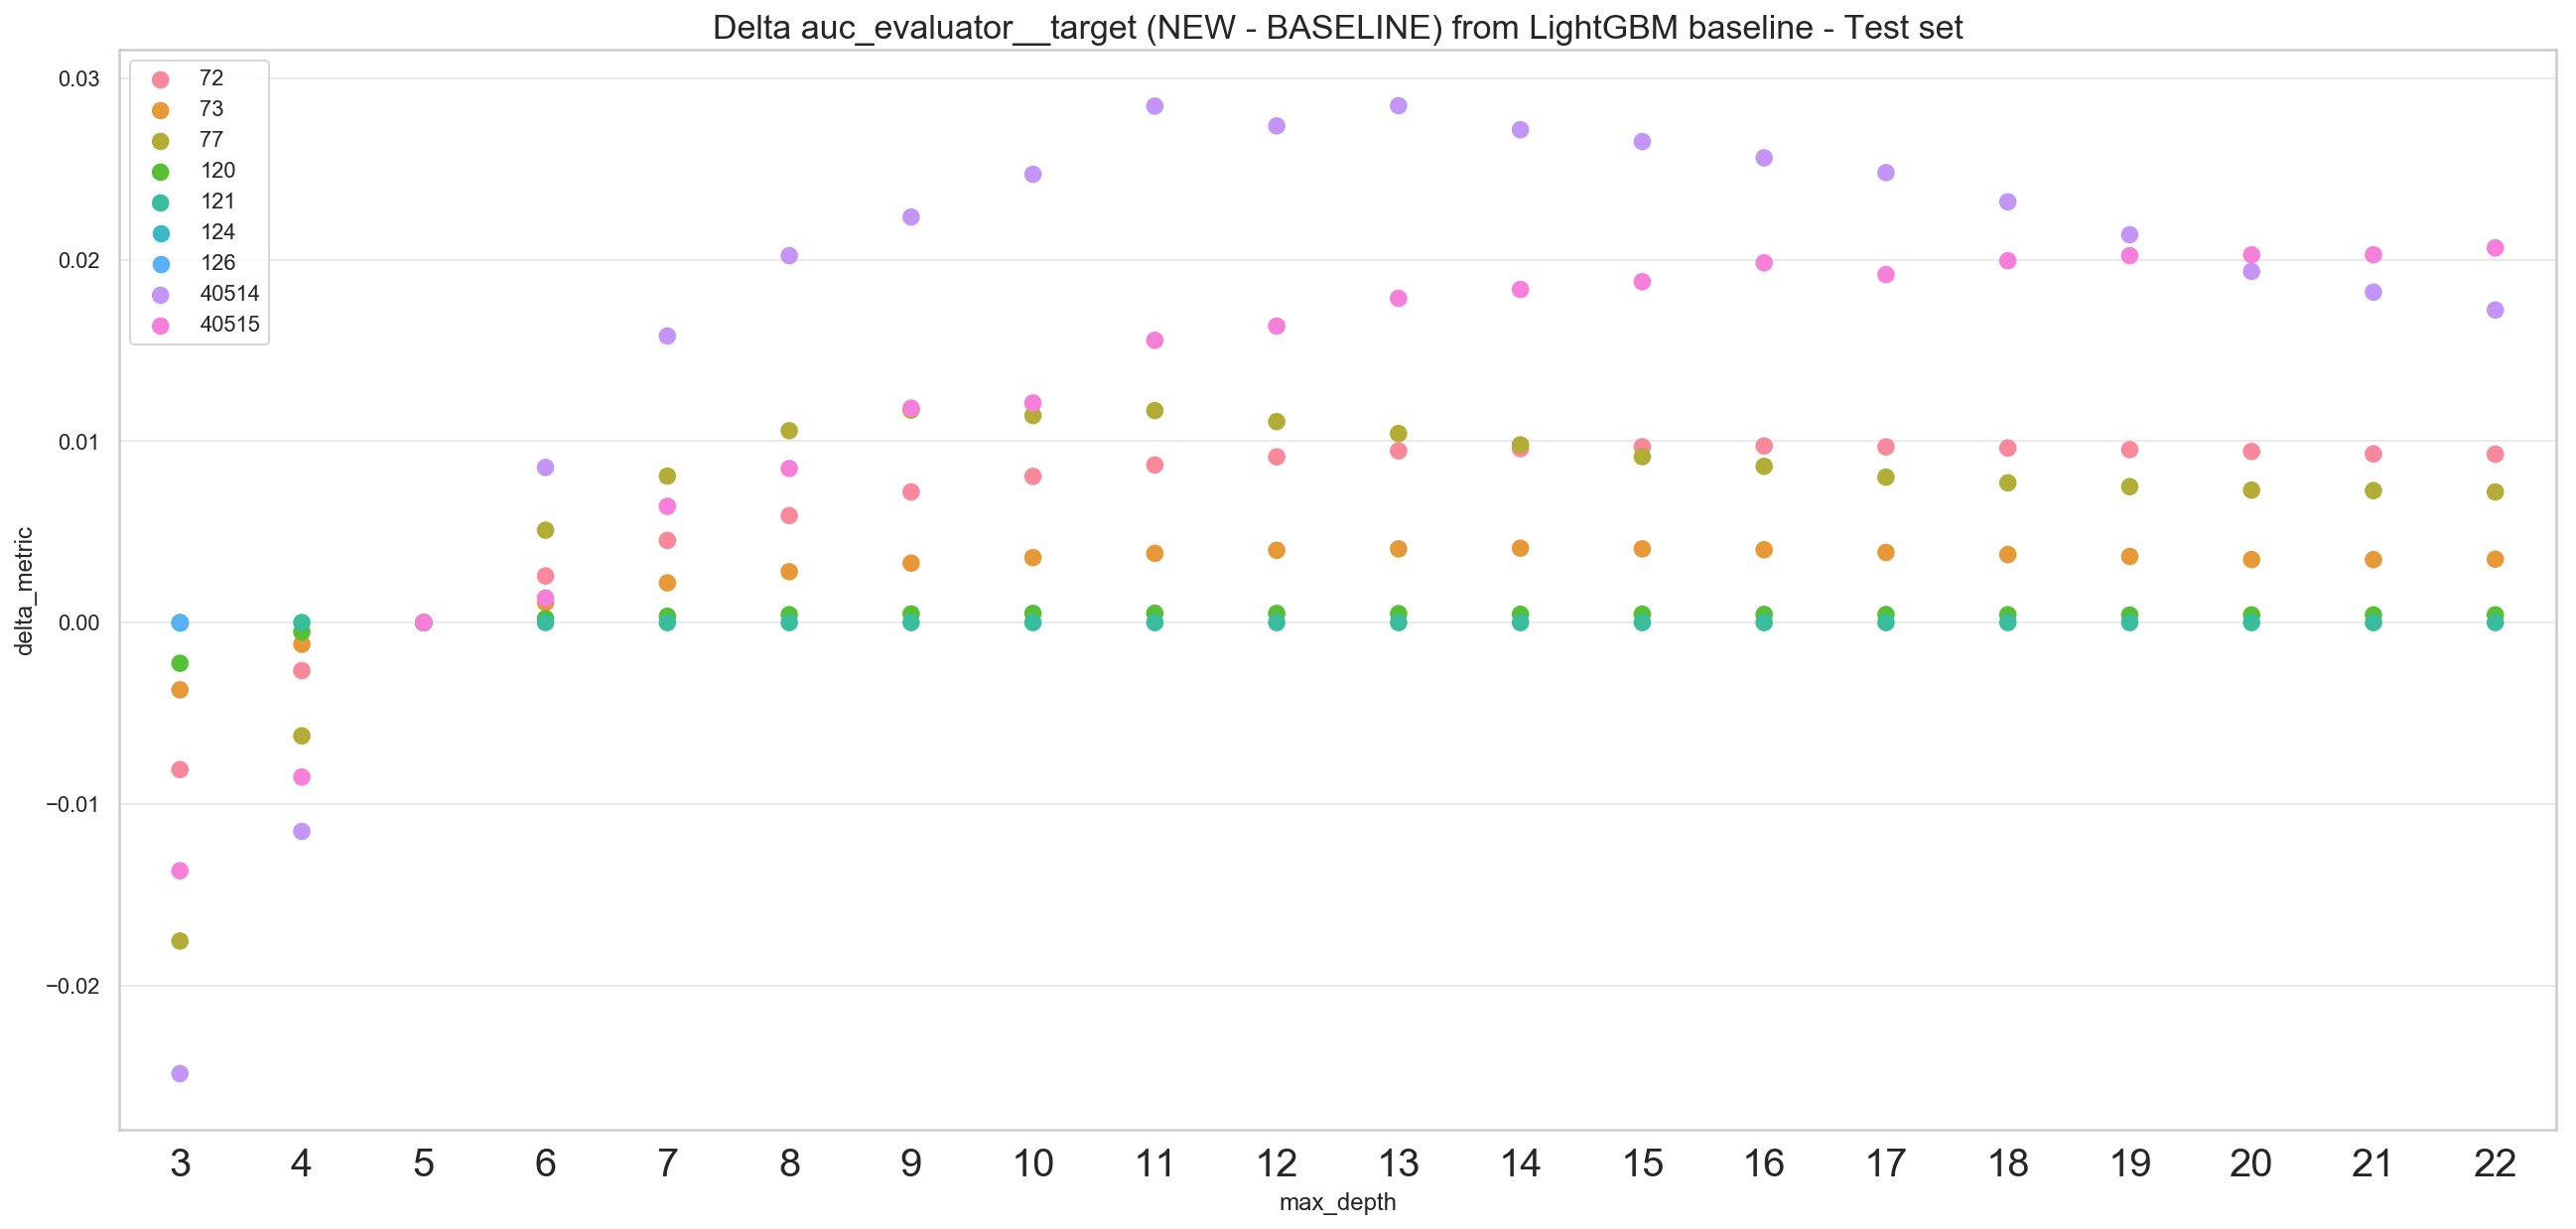
\includegraphics[width=1\textwidth]{delta_auc1.png}
    \caption{$\delta_{AUC}$ for Cluster 3, changing only \code{max\_depth}. The colors represent different datasets}
    \label{fig:delta-auc1}
\end{figure}

\subsection{Ordering and Visualization}
\label{subsec:ordering}

In Figure \ref{fig:delta-brier1} a different $\delta_{metric}$ plot is displayed, where each point is the $\delta_{brier}$ w.r.t both \code{max\_depth} and \code{learning\_rate} changes summarized into a single dimension in the \textit{x-axis}, for Cluster 2 experiments. The higher the number of hyperparameters being analyzed at the same time, the more difficult it is to visualize these $\delta_{metric}$ plots due to the high dimensionality. For this reason, in the study the hyperparameter values were summarized into a single point that encompasses multiple hyperparameter changes.

\begin{figure}[!h]
    \centering
    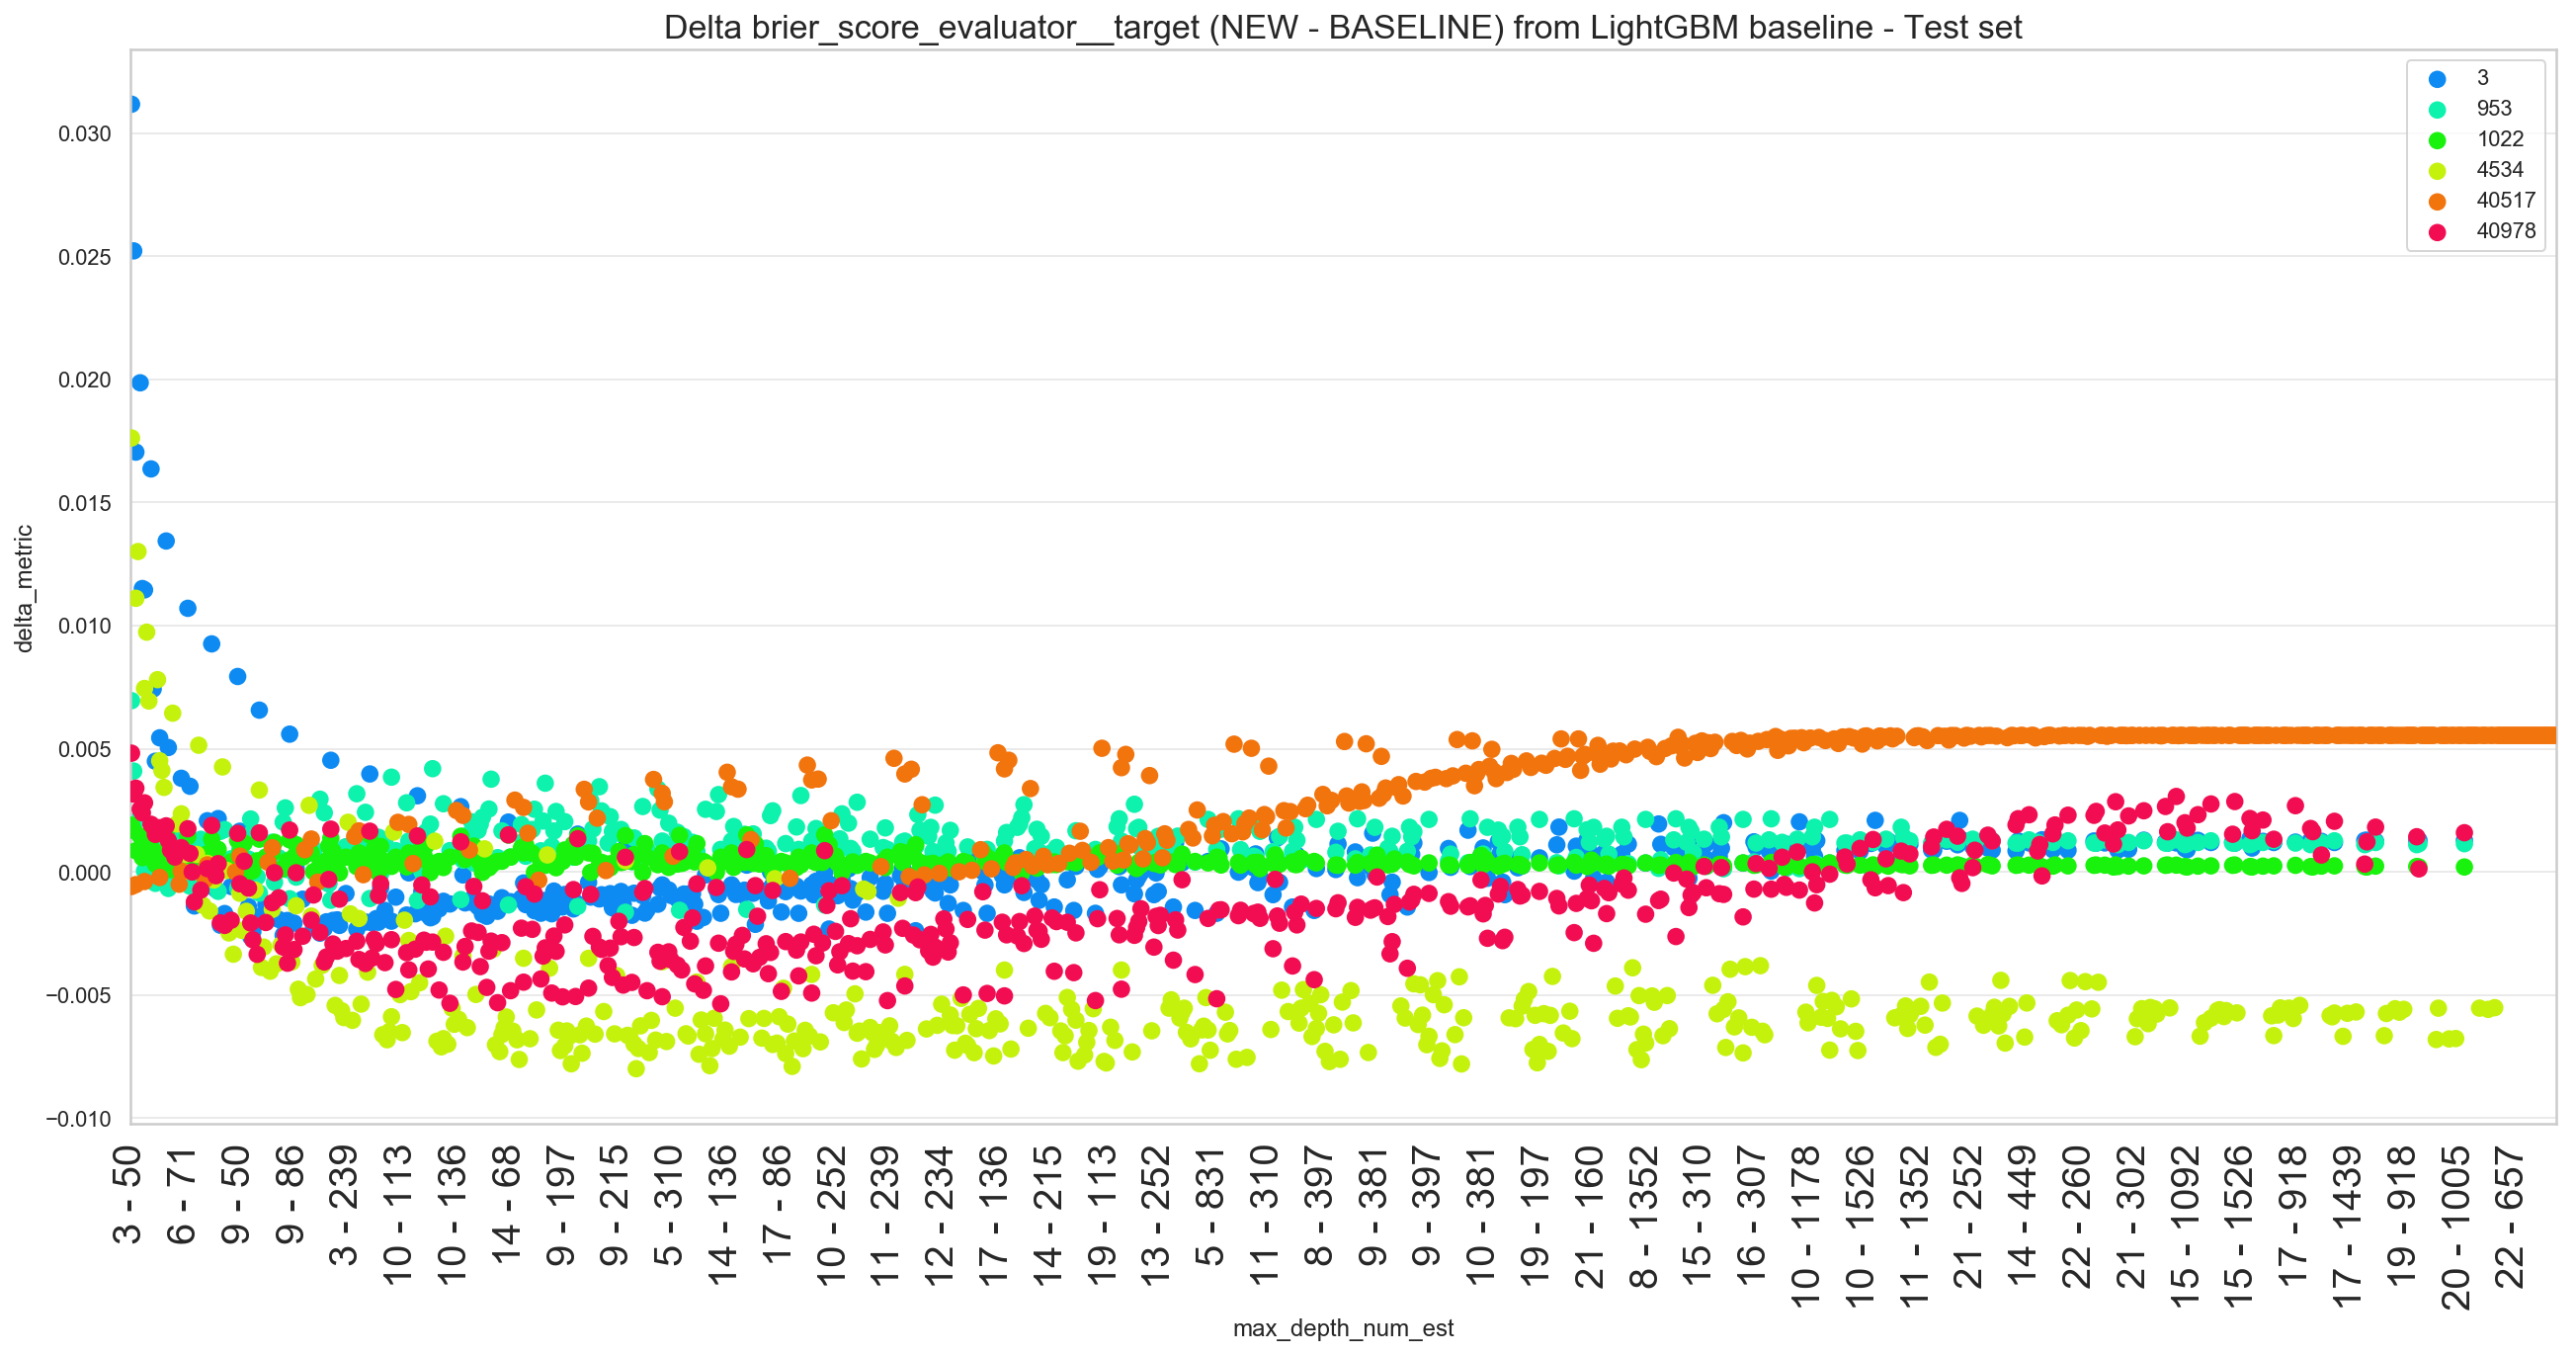
\includegraphics[width=1\textwidth]{delta_brier1.png}
    \caption{$\delta_{Brier}$ for Cluster 2, changing both \code{max\_depth} and \code{learning\_rate}. The colors represent different datasets}
    \label{fig:delta-brier1}
\end{figure}


In the Subsections \ref{subsec:indv-impact}, \ref{subsec:double-impact} and \ref{subsec:triple-impact} it is shown the full results for individual hyperparameter impact, pairs of hyperparameters and finally all three hyperparameters, respectively. These plots are not possible in this part of the analysis because instead of one individual dataset experiment result being evaluated as in Section \ref{sec:single-dataset}, the final analysis is done with multiple datasets of a cluster.

For visualization purposes, an ordering of the data points in the x-axis was defined to facilitate the visualization and to maintain an order that makes sense, even when reducing the dimensionality. First, the ranking of each hyperparameter is calculated based on the sorted order within that individual hyperparameter distribution, and then the final ranking of these points is based on the average of the individual hyperparameter ranks. This custom ranking has two advantages:

\begin{enumerate}
    \item Retains the relative value of each hyperparameter into the final ordering. This means that the first points represent the lower values of all hyperparameters and the last points in the x-axis represent the combinations with the highest hyperparameters values;
    \item Is robust w.r.t the scale of the absolute values between the hyperparameters. The ordering takes first into account the rank of each hyperparameter to avoid dealing with values in uneven scales. For example, a learning rate of $1.5$ is considered to be a high value in practice, but its numeric value is much smaller than a maximum depth of $5$, which can be considered a small value of \code{max\_depth}.
\end{enumerate}


As an example of this ordering, if the points were $H = \{(3, 500), (20, 100), (5, 200), (10, 400)\}$, each tuple a 
pair of maximum depth and number of estimators, the first step of the ordering is to get the ranking of each hyperparameter within it is distribution. This would generate a set of the individual ranks $r'(H) = \{(1, 4), (4, 1), (2, 2), (3, 3)\}$, and the final ranking order depends on the average ranks of each tuple, in this case $r_{avg}(H) = \{2.5, 2.5, 2, 3\}$. And using $r_{avg}(H)$ to order the original points $H$, the final ordering is $H^\star = \{(5, 200), (3, 500), (20, 100), (10, 400)\}$.

it is important to note that, because of the statistical framework chosen in the study, the ranking strategy does not change the result of the analysis, but provides a way to visually understand its results.

%% ------------------------------------------------------------------------- %%
\section{Statistical Framework}

To generalize and be more certain about the hyperparameter sensitivity analysis, a statistical framework is defined to analyze the $\delta_{metric}$ obtained on each cluster and different configurations of hyperparameters. The comparisons include changing different aspects of the experiment, such as the performance metric chosen (AUC, Logloss, Brier Score), the hyperparameter(s) being changed and the clusters being analyzed.

The statistical framework is divided into two main parts: tests for the significance of the changes in the $\delta_{metric}$ obtained in the experiment, and the subsequent modeling of the sensitivity factors of the hyperparameters of each cluster. An overview of the statistical tools used is defined in the following subsections, along with examples of real results obtained in the analysis of the experiments.

\subsection{Experimental Scenarios}

An important concept in this study related to the statistical framework is the definition of an \textbf{experimental scenario}. In this study the experimental units are the datasets of a cluster, which receive a "treatment" of different hyperparameter values. First, $C_k$ is the set of experimental units (i.e. the datasets) of the $k$th cluster. The hyperparameters of a scenario are a partition $Q$ of the union of all hyperparameter spaces (as defined in Subsection \ref{subsec:hp-tree}) of the $k$th cluster ($\eta^{(k)}$, defined in Equation \ref{eq:exp-Hspace}) and is referred to as  $\eta^{(k)}_Q$. For example, the hyperparameters values of the experiment when changing both maximum depth and learning rate in Cluster 4 can be written as $\eta^{(4)}_{max\_depth, learning\_rate}$.

\begin{equation}
    \eta^{(k)} = \bigcup_{d \in C_k} Hspace_d
    \label{eq:exp-Hspace}
\end{equation}


\noindent Given the $C_k$ experimental units, the hyperparameters configuration  $\eta^{(k)}_Q$ and a performance metric $m$, the experimental scenario can be represented as is Equation \ref{eq:exp-scenario}:

\begin{equation}
 \mathcal{S}(C_k, \eta^{(k)}_Q, m)
 \label{eq:exp-scenario}
\end{equation}

\noindent Which means the experiment outputs of $\delta_m$ observed when applying the \textit{treatments} $\eta^{(k)}_Q$ to all experimental units in the $k$th cluster. For example,  Figure  \ref{fig:delta-auc1} represents the experimental scenario $\mathcal{S}(C_3, \eta^{(3)}_{max\_depth}, AUC)$ and Figure  \ref{fig:delta-brier1} is a visualization of $\mathcal{S}(C_2, \eta^{(2)}_{max\_depth,num\_estimators}, brier)$.


\subsection{Analysis of Variance}

The typical scenario of an analysis of variance, according to \cite{montgomery2017design}, is an experimental setting where there are $k$ {treatments} or different \textit{levels} of a factor that one wishes to compare. The response observed from each of the $k$ levels of treatment is a random variable. In general, there are $n$ observations under the same treatment, which can be seen in Table \ref{table:sfm}. In this study, the \textit{treatment} is the hyperparameter, and the different values of the hyperparameter are the different treatment levels in the analysis of variance.

\begin{table}[H] 
    \centering
    \begin{tabular}{||c |c c c c| c c||} 
     \hline
     \textbf{Treatment} & & \textbf{Observations} & & & \textbf{Totals} & \textbf{Averages} \\ [0.5ex]
     \hline
     $1$ & $y_{11}$ & $y_{12}$ & $\cdots$ & $y_{1n}$ & $\bm{y}^{(1)}$ & $\overline{\bm{y}^{(1)}}$\\
     $2$ & $y_{21}$ & $y_{22}$ & $\cdots$ & $y_{2n}$ & $\bm{y}^{(2)}$ & $\overline{\bm{y}^{(2)}}$\\
     $\vdots$ & $\vdots$ & $\vdots$ & $\cdots$ & $\vdots$ & $\vdots$ & $\vdots$\\
     $k$ & $y_{k1}$ & $y_{k2}$ & $\cdots$ & $y_{kn}$ & $\bm{y}^{(k)}$ & $\overline{\bm{y}^{(k)}}$\\[1ex]
     & &  &  &  &\text{\Large$\mathup{y}_\Sigma$} & \text{\Large$\overline{\mathup{y}_\Sigma}$}\\[1ex] 
     \hline
    \end{tabular}
    \caption{Table exemplifying a general Single-Factor Experiment, based on \cite{montgomery2017design}}
    \label{table:sfm}
\end{table}

There are two main models in the literature when dealing with Single-Factor experiments, the \textbf{means model} and the \textbf{effects model}. Even though in this study the observations from the experiments are described using the \textit{effects model}, it is useful to comprehend the idea behind both models to understand why one was chosen over the other.

In the \textit{means model} each observation (i.e. each point in the $\delta_{metric}$ plot for example) is defined as a function of the mean \textit{within treatment} and a random error component that incorporates ``all other sources of variability in the experiment including measurement, variability arising from uncontrolled factors, differences between the experimental units to which the treatments are applied, and the general background noise in the process'' according to \cite{montgomery2017design}. The structure from the means model is described in Equation \ref{eq:means-model}.

\begin{equation}\label{eq:means-model}
    y_{ij} = \mu_i + \epsilon_{ij}
    \begin{cases}
        i = 1, 2, \cdots , k\\
        j = 1, 2, \cdots, n
    \end{cases}
\end{equation}

On the other hand, the \textbf{effects model} defines the treatment means $\mu_i$ as a deviation from the overall mean $\bm{\mu}$ of the experiment, i.e. $\mu_i = \bm{\mu}+ \tau_i \text{ where } i = 1, 2, \cdots, k$. Thus, the experimental results are described according to Equation \ref{eq:effects-model}. The parameter $\tau_i$ is called the \textbf{\textit{i}th treatment effect}, and it represents the deviation from the overall mean of the experiment.

For simplicity, all the scenarios were structured using a single-factor model, even the scenarios where the treatment is actually two or more values of different hyperparameters being changed. This means that the results and conclusions from pairs or triples of hyperparameters are interpreted as a single factor that can change the $\delta_{metric}$ of the gradient boosting models, instead of decomposing the effects into multiple variables.

\begin{equation}\label{eq:effects-model}
    y_{ij} = \bm{\mu} + \tau_i + \epsilon_{ij}
    \begin{cases}
        i = 1, 2, \cdots , k\\
        j = 1, 2, \cdots, n
    \end{cases}
\end{equation}

One of the reasons why the effects model was chosen to analyze the results of this study is because it has a more intuitive interpretation for the objective of this study. One can interpret the $\tau_i$ as the amount of effect a configuration of hyperparameter produces in the performance metrics, i.e. It is a measure of textit{sensitivity} from the overall case. Before modeling the experimental results and comparing the $\tau_i$ for different scenarios, it is important to test for equality of the output of the treatments (in this case, equality of $\delta_{metric}$ for different performance metrics) and testing the assumptions of the statistical tests.

\subsection{ANOVA}

The most widely used test in the analysis of variance is the \textbf{ANOVA} test or \textit{single-factor analysis of variance}. In the assumptions of the ANOVA model, there is a requirement that the experiments are performed in random order to keep the environment in which the experiments are applied as uniform as possible. According to \cite{montgomery2017design}, the objective is to test the appropriate hypothesis about the treatment means and to estimate them. However, there a very strong assumption that must be validated before applying the ANOVA test: the model errors $\epsilon_{ij}$ are assumed to be normally and independently distributed random variables with mean zero and variance $\sigma^2$; The data must also be \textit{homoscedastic}, i.e. the variance $\sigma^2$ is assumed to be constant for all levels of the factor.

These assumptions imply that the observations must follow a normal distribution:

$$y_{ij} \sim \mathcal{N}(\bm{\mu} + \tau_i, \sigma^2)$$

The ANOVA model has different flavors, and is highly used in the field of applied statistics. Different variations and extensions of the ANOVA model can be found throughout the literature of statistics and machine learning. In the study of hyperparameters, \cite{hoos201x4efficient} describes a method using the functional ANOVA framework (a variation of ANOVA) to quantify the importance of ``both single hyperparameters and of interactions between hyperparameters'' in a single dataset. In more recent work, \cite{van2017empirical} also extends the functional ANOVA framework for multiple datasets, with an empirical experiment using OpenML datasets.

\subsection{Testing of Assumptions}

However, the ANOVA test \textbf{was not} used in this study, because its assumptions were not met in almost all scenarios. A different nonparametric statistical test was used, and since some of the assumptions apply for both the parametric (ANOVA) and nonparametric tests, it is important to understand the assumptions of them. Using \cite{montgomery2017design} definition of the \textbf{residuals} for observation $j$ in treatment $i$ as

\begin{equation}
    \mathcal{E}_{ij} = y_{ij} - \hat{y}_{ij}    
    \label{eq:sfm-residuals}
\end{equation}


\noindent where $\hat{y}_{ij}$ is an estimate of the respective observation $y_{ij}$, obtained as follows:

\begin{equation}    
    \begin{split}
        \hat{y}_{ij} & = \hat{\bm{\mu}} + \hat{\tau_i}\\
        & = \text{\Large$\overline{\mathup{y}_\Sigma}$} + (\overline{\bm{y}^{(i)}} - \text{\Large$\overline{\mathup{y}_\Sigma}$})\\
        & = \overline{\bm{y}^{(i)}}
    \end{split}
\end{equation}

\noindent This just means that the estimate of any experimental scenario observation in the $i$th treatment is the corresponding treatment average $\overline{\bm{y}^{(i)}}$. In the terms of this study, the estimate of relative change in the performance metric $\delta_{metric}$ for a given configuration of a value of hyperparameters is the mean of the $\delta_{metric}$'s of all datasets in the corresponding cluster being analyzed. The analysis of the residuals is one of the ways to check for model adequacy, and can be analyzed using a \textit{Normal Q-Q Plot} and using statistical tests to test for the normality and homoscedasticity assumptions.

The test of assumptions is applied to every \textbf{experimental scenario} $\mathcal{S}$ in this study, in the following order:
\newpage
\begin{enumerate}
    \item Fit a single-factor model (SFM) on $\mathcal{S}$, and calculate the residuals according to Equation \ref{eq:sfm-residuals}. In Table \ref{table:sfm-cluster1} the complete SFM model output for $\mathcal{S}(C_1, \eta^{(1)}_{max\_depth}, Brier)$ is illustrated.
    \begin{table}[!h]
        \centering
        \begin{tabular}{lrrr}
            \toprule
            {} &  $\overline{\bm{y}^{(i)}}$ &  $ \hat{\bm{\mu}}$ & $ \hat{\tau_i}$  \\
            max\_depth &                 &          &             \\
            \midrule
            3         &        0.001872 & -0.00106 &    0.002932 \\
            4         &        0.001275 & -0.00106 &    0.002335 \\
            5         &        0.000000 & -0.00106 &    0.001060 \\
            6         &       -0.000835 & -0.00106 &    0.000225 \\
            7         &       -0.001350 & -0.00106 &   -0.000290 \\
            8         &       -0.001588 & -0.00106 &   -0.000528 \\
            9         &       -0.001548 & -0.00106 &   -0.000488 \\
            10        &       -0.001575 & -0.00106 &   -0.000515 \\
            11        &       -0.001558 & -0.00106 &   -0.000497 \\
            12        &       -0.001646 & -0.00106 &   -0.000586 \\
            13        &       -0.001451 & -0.00106 &   -0.000391 \\
            14        &       -0.001456 & -0.00106 &   -0.000396 \\
            15        &       -0.001413 & -0.00106 &   -0.000352 \\
            16        &       -0.001397 & -0.00106 &   -0.000337 \\
            17        &       -0.001391 & -0.00106 &   -0.000331 \\
            18        &       -0.001425 & -0.00106 &   -0.000365 \\
            19        &       -0.001395 & -0.00106 &   -0.000335 \\
            20        &       -0.001383 & -0.00106 &   -0.000323 \\
            21        &       -0.001439 & -0.00106 &   -0.000379 \\
            22        &       -0.001501 & -0.00106 &   -0.000441 \\
            \bottomrule
            \end{tabular}
        \caption{SFM model for scenario $\mathcal{S}(C_1, \eta^{(1)}_{max\_depth}, Brier)$}
        \label{table:sfm-cluster1}
        \end{table}
        
    
    \item Plot a Normal Q-Q Plot to visually observe the structure of the SFM residuals. In this study, the Normal Q-Q Plot will match the SFM residuals quantiles with the theoretical quantiles of a normal distribution, while also fitting a Linear Regression model and calculating the coefficient of determination ($R^2$), as suggested in \cite{Vallat2018}. Residuals are filtered to be inside the quantiles $q_{5}$ and $q_{95}$ to remove outliers. To showcase this, in Figure \ref{fig:resplot-1} the Normal Q-Q plot for the scenario $\mathcal{S}(C_1, \eta^{(1)}_{max\_depth, learning\_rate}, AUC)$ represents a distribution of residuals close to a normal distribution, with a relatively high $R^2$. This is a specific case where the ANOVA test could be used because of its robustness to the normality assumption, as stated in \cite{montgomery2017design} ``In general, moderate departures from normality are of little concern in the fixed effects analysis of variance''. A more drastic departure from normality can be observed in scenario $\mathcal{S}(C_1, \eta^{(1)}_{num\_estimators, learning\_rate}, Logloss)$, in Figure \ref{fig:resplot-2}.
    \begin{figure}[H]
        \centering
        \begin{subfigure}[b]{0.8\textwidth}
            \centering
            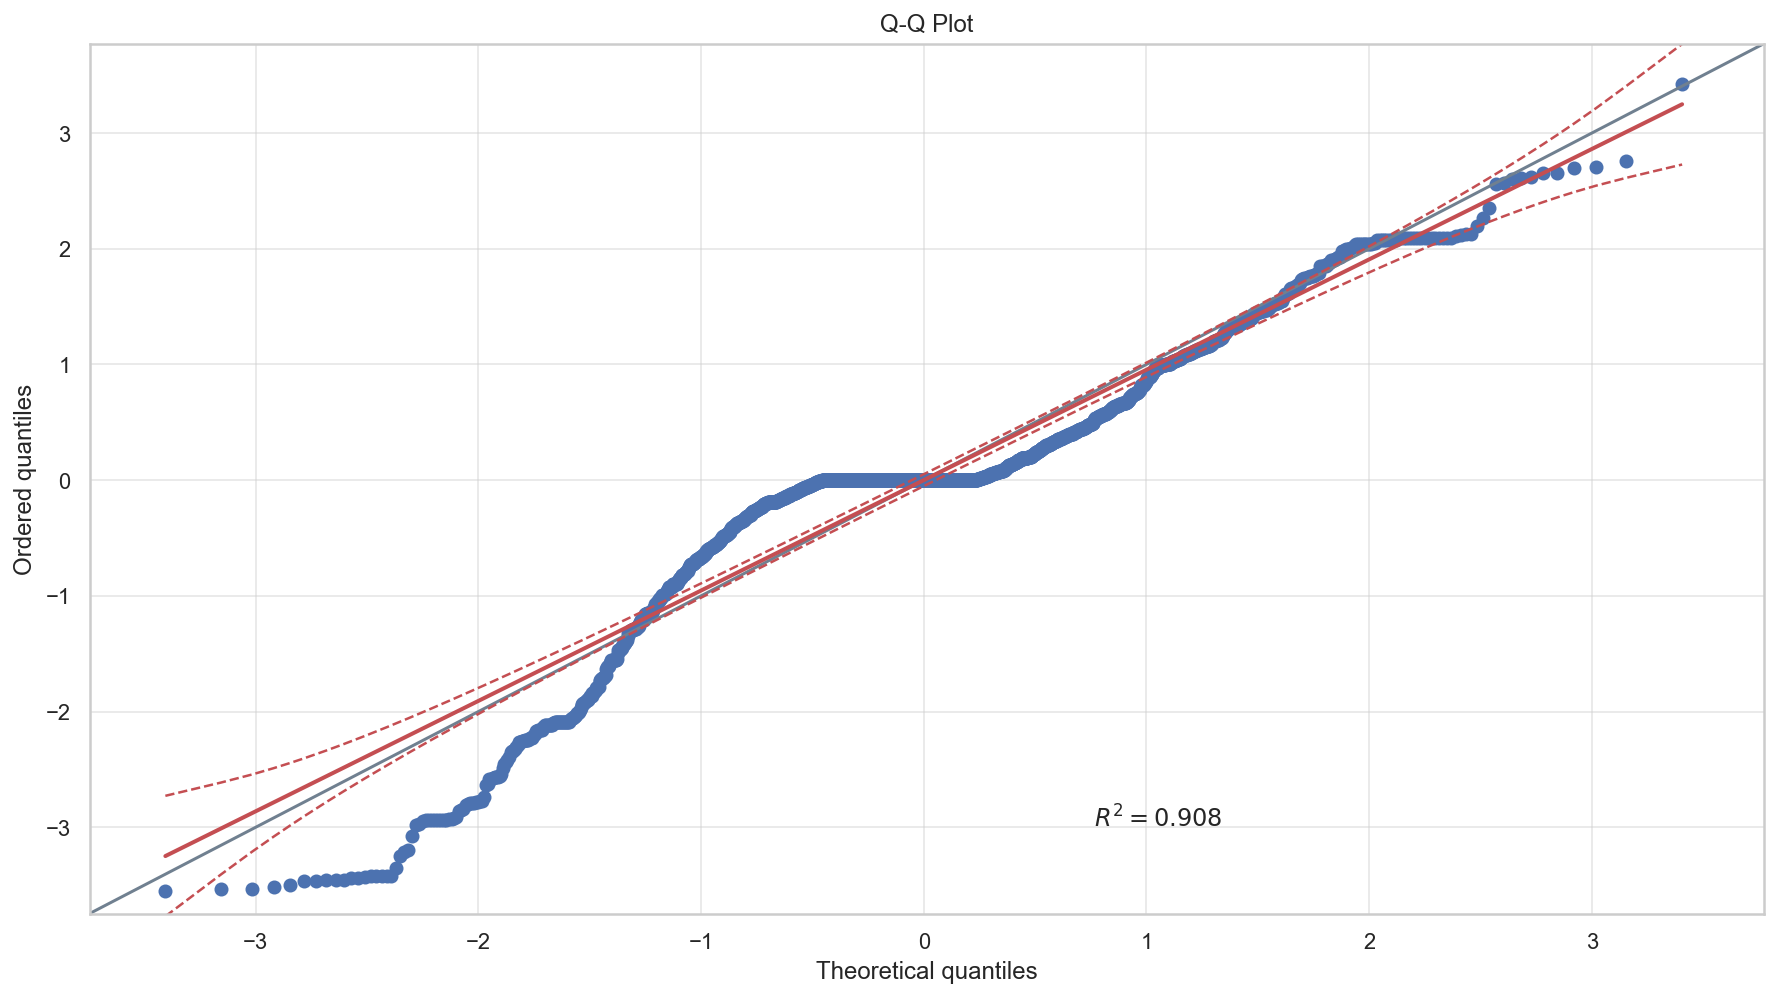
\includegraphics[width=\textwidth]{qqplot_c1.png}
            \caption{Normal Q-Q Plot for scenario $\mathcal{S}(C_1, \eta^{(1)}_{max\_depth, learning\_rate}, AUC)$}
            \label{fig:resplot-1}
        \end{subfigure}
        \hfill
        \begin{subfigure}[b]{0.8\textwidth}
            \centering
            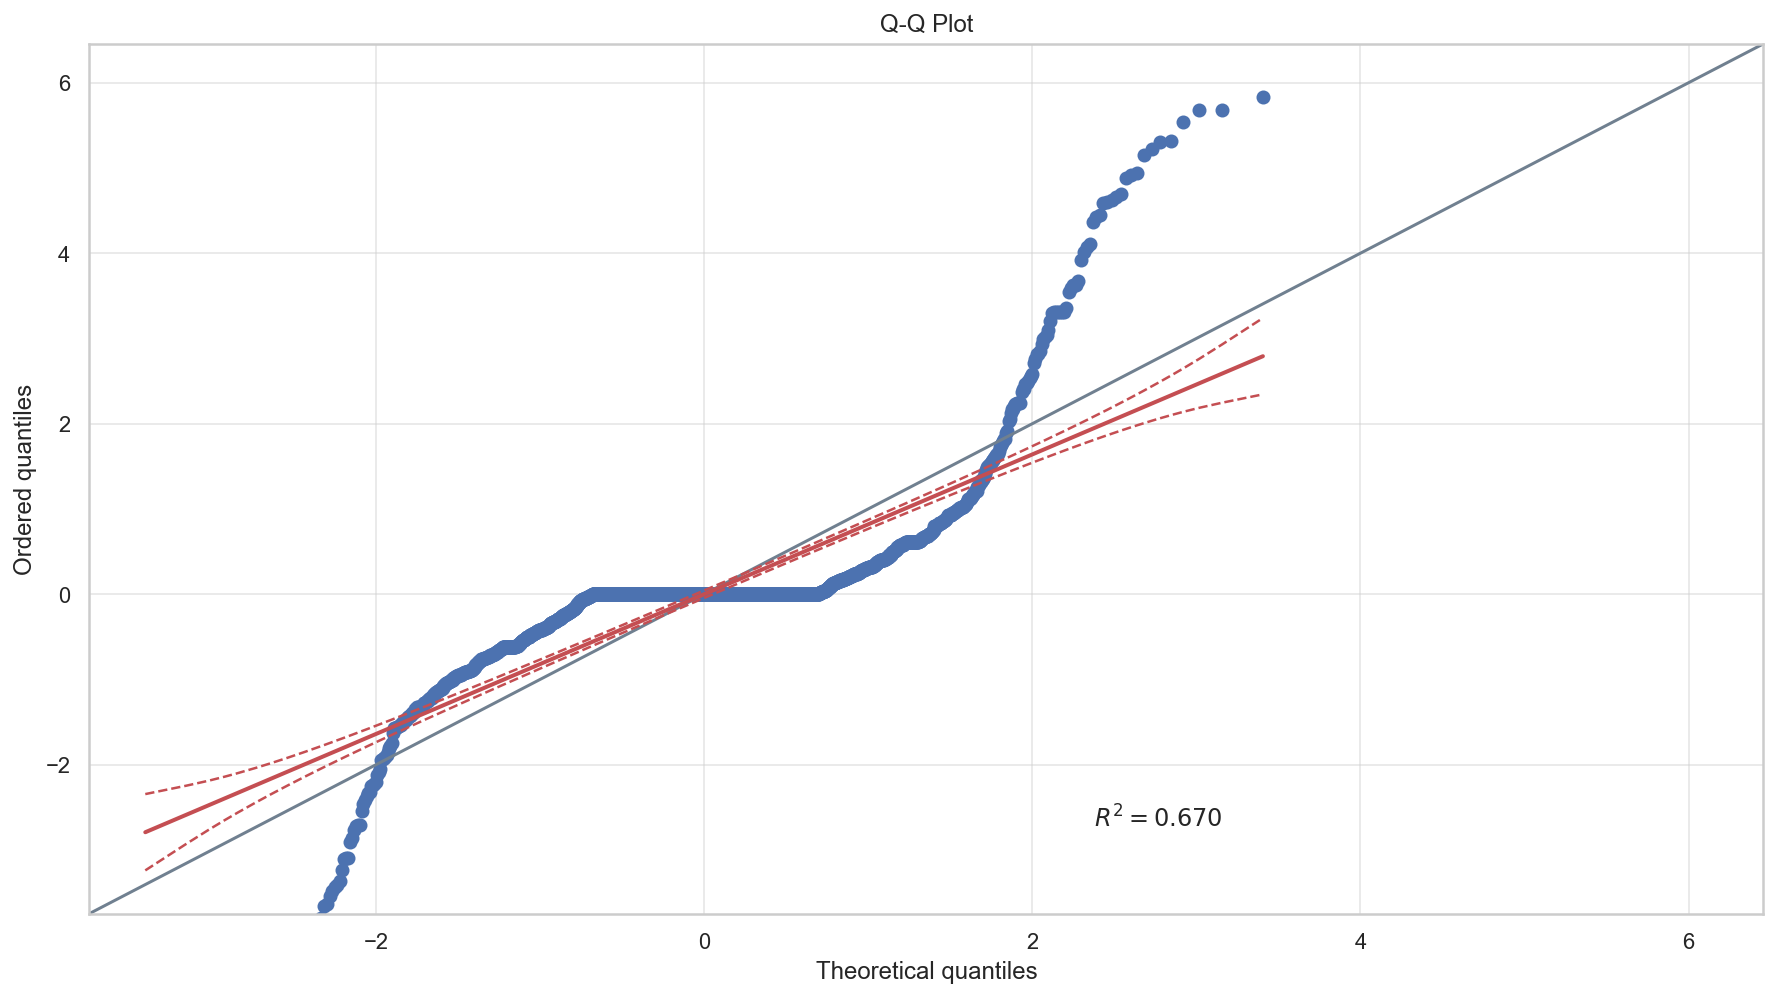
\includegraphics[width=\textwidth]{qqplot_c1_bad.png}
            \caption{Normal Q-Q Plot for scenario $\mathcal{S}(C_1, \eta^{(1)}_{num\_estimators, learning\_rate}, Logloss)$}
            \label{fig:resplot-2}
        \end{subfigure}
        \hfill
           \caption{Two Normal Q-Q Plots from Cluster 1 results}
           \label{fig:three graphs}
   \end{figure}
       
    \item Perform a {\large\textbf{Shapiro–Wilk test}} for the normality assumption with $\alpha\text{-level} = 0.05$. In almost all of the experimental scenarios the test rejected the null hypothesis that the residuals are normally distributed with $p$-value less than $0.05$.

    \item To validate the homoscedasticity assumption, a statistical test for equality of variance is also performed on the residuals. As indicated in \cite{montgomery2017design}, these statistical procedures are testing the following hypotheses:
    \begin{align*}
        H_0 &: \sigma^2_1 =  \sigma^2_2 = \cdots =  \sigma^2_k \\
        H_1 &: \text{above not true for at least one } \sigma^2_i    
    \end{align*}
    A widely used procedure for homoscedasticity is the Bartlett's Test, which computes a statistic whose sampling distribution is, according to \cite{montgomery2017design}: ``closely approximated by the chi-square distribution with $k - 1$ degrees of freedom when the $k$ random samples are from independent normal populations.''. By analyzing the results of the Normal Q-Q plots and the Shapiro–Wilk tests there is no statistical evidence that the residuals of this study follow a normal distribution, so the Bartlett's test should not be used.
    The {\large\textbf{Levene test}} is an alternate procedure that is robust to departures from normality, as explained in \cite{brown1974robust}, and it is the test chosen to verify the homoscedasticity for all experimental scenarios.
    
\end{enumerate}

\subsection{Kruskal–Wallis: A Nonparametric Approach}

Given that most of the experimental results failed the normality assumption tests, the Kruskal–Wallis test is used to test for the statistical significance of the treatment means. The Kruskal–Wallis test is applied to all experimental scenarios and is used to test the null hypothesis that the $k$ treatments are identical against the alternative hypothesis that some of the treatments generate observations that are larger than others. There is a convenient interpretation of the Kruskal–Wallis, described in \cite{montgomery2017design}:

\begin{displayquote}

``Because the procedure is designed to be sensitive for testing differences in means, it is sometimes convenient to think of the Kruskal–Wallis test as a test for equality of treatment means. The Kruskal–Wallis test is a \textbf{nonparametric alternative} to the usual analysis of variance.''

\end{displayquote}

Kruskal–Wallis works by applying the usual analysis of variance to the ranks of the observations. The \textit{rank transformation} consists of ranking the observations $y_{ij}$ in ascending order and replacing each observation by its rank $r_{ij}$. The results of testing after a ranking transformation are preferred because it is less likely to be distorted by nonnormality and unusual observations, which is the case of the results of the experimental scenarios in the study.

Even though this nonparametric approach does not require the data to be normally distributed, it does, however, assume the same distribution within groups, as explained in \cite{mcdonald2009handbook}:

\begin{displayquote}
    ``(Kruskal–Wallis) does assume that the different groups have the same distribution, and groups with different standard deviations have different distributions. If your data are heteroscedastic, Kruskal–Wallis is no better than one-way ANOVA, and may be worse.''
\end{displayquote}

So the homoscedasticity tests are still needed for the assumptions of the Kruskal–Wallis test. In Table \ref{table:result-cluster2} the statistical results for all the scenarios in Cluster 2 is available, where $NE$, $MD$ and $LR$ refer to \code{num\_estimators}, \code{max\_depth} and \code{learning\_rate} respectively. The numbers in the table are the $p$-values of all statistical tests performed in Cluster 2 experiments, and the values in \textcolor{red}{red} are the tests that failed the desired hypothesis testing. Some tests can have NaN if there are not enough samples or all values are equal, in the case of the residuals.

\begin{table}[!h]
    \centering
    \begin{tabular}{l|lrrr}
        \toprule
                             &         &       Shapiro–Wilk &        Levene &        Kruskal–Wallis \\
        \textbf{Treatment} & \textbf{Metric} &               &               &                \\
        \midrule
        $\eta^{(2)}_{NE}$ & $\delta_{AUC}$ &  \textcolor{red}{4.059920e-08} &  9.968117e-01 &   \textcolor{red}{9.996506e-01} \\
                             & $\delta_{Brier}$ &  \textcolor{red}{5.942564e-06} &  2.105453e-01 &   \textcolor{red}{9.965572e-01} \\
                             & $\delta_{Logloss}$ &  \textcolor{red}{2.502680e-05} &  \textcolor{red}{9.636175e-03} &   2.827828e-03 \\
                             \hline
        $\eta^{(2)}_{MD}$ & $\delta_{AUC}$ &  \textcolor{red}{2.536182e-10} &  9.210022e-01 &   1.860650e-02 \\
                             & $\delta_{Brier}$ &  \textcolor{red}{3.926061e-06} &  2.774635e-01 &   2.283747e-02 \\
                             & $\delta_{Logloss}$ &  \textcolor{red}{2.522154e-05} &  1.285176e-01 &   1.764531e-02 \\
                             \hline
        $\eta^{(2)}_{LR}$ & $\delta_{AUC}$ &  \textcolor{red}{2.714980e-09} &           NaN &            NaN \\
                             & $\delta_{Brier}$ &  \textcolor{red}{9.808685e-09} &           NaN &            NaN \\
                             & $\delta_{Logloss}$ &  \textcolor{red}{1.213540e-10} &           NaN &            NaN \\
                             \hline
        $\eta^{(2)}_{MD, LR}$ & $\delta_{AUC}$ &  \textcolor{red}{1.406702e-20} &  9.999939e-01 &   1.316980e-02 \\
                             & $\delta_{Brier}$ &  \textcolor{red}{1.339994e-23} &  1.000000e+00 &   6.235464e-12 \\
                             & $\delta_{Logloss}$ &  \textcolor{red}{1.334960e-23} &  1.000000e+00 &   1.005025e-08 \\
                             \hline
       $\eta^{(2)}_{MD, NE}$ & $\delta_{AUC}$ &  \textcolor{red}{2.548462e-22} &  1.000000e+00 &   \textcolor{red}{1.000000e+00} \\
                             & $\delta_{Brier}$ &  \textcolor{red}{6.494320e-28} &  9.969882e-01 &   \textcolor{red}{9.274816e-01} \\
                             & $\delta_{Logloss}$ &  \textcolor{red}{3.974093e-21} &  \textcolor{red}{2.655356e-23} &   6.191510e-22 \\
                             \hline
        $\eta^{(2)}_{LR, NE}$ & $\delta_{AUC}$ &  \textcolor{red}{9.960932e-27} &  1.000000e+00 &   3.306332e-06 \\
                             & $\delta_{Brier}$ &  \textcolor{red}{2.709085e-26} &  9.999995e-01 &   7.035798e-09 \\
                             & $\delta_{Logloss}$ &  \textcolor{red}{2.452305e-24} &  9.999999e-01 &   1.650304e-05 \\
                             \hline
        $\eta^{(2)}_{NE, MD, LR}$ & $\delta_{AUC}$ &  \textcolor{red}{0.000000e+00} &  1.000000e+00 &   2.904172e-64 \\
                             & $\delta_{Brier}$ &  \textcolor{red}{0.000000e+00} &  1.000000e+00 &  4.013155e-111 \\
                             & $\delta_{Logloss}$ &  \textcolor{red}{0.000000e+00} &  1.000000e+00 &   7.298816e-70 \\
        \bottomrule
\end{tabular}        
\caption{Statistical $p$-values of the experimental scenarios in Cluster 2. All the normality assumptions were rejected in this case}
\label{table:result-cluster2}
\end{table}
